\documentclass[10pt,a4j,dvipdfmx]{jarticle}
%---------------------------------------------------
\usepackage{hyperref}
\usepackage{pxjahyper}
\usepackage{bm}
\usepackage{graphicx}
\usepackage{amssymb,amsmath}
\usepackage{ascmac}
\usepackage{float}
\usepackage{setspace}
\usepackage[dvips,usenames]{color}
\usepackage{colortbl}
\usepackage{algorithm}
\usepackage{algorithmic}
\usepackage{setspace}
\usepackage{subfigure}
\usepackage{here}
\usepackage[deluxe,bold]{otf}
\usepackage[haranoaji]{pxchfon}
\usepackage{redeffont}
\usepackage{listings,jvlisting} %日本語のコメントアウトをする場合jvlisting(もしくはjlisting)が必要
\usepackage{booktabs}
\usepackage{siunitx} %SI単位
\usepackage{fancybox}
%---------------------------------------------------
% \definecolor{bl}{rgb}{0.94,0.97,1}
% \definecolor{gr}{rgb}{0.5,0.5,0.5}
% \makeatletter
% \def\section{\newpage\@startsection {section}{1}{\z@}{2.3ex plus -1ex minus -.2ex}{2.3 ex plus .2ex}{\Large\bfseries}}
% \makeatother
%---------------------------------------------------
\setlength{\textwidth}{160truemm}
\setlength{\textheight}{240truemm}
\setlength{\topmargin}{-14.5truemm}
\setlength{\oddsidemargin}{-0.5truemm}
\setlength{\headheight}{0truemm}
\setlength{\parindent}{1zw}
\setlength{\abovedisplayskip}{-2pt} % 数式上部のマージン
\setlength{\belowdisplayskip}{-2pt} % 数式下部のマージン
%---------------------------------------------------
\setstretch{1.2}
%---------------------------------------------------
\renewcommand{\subfigtopskip}{5pt}	% 図の上の隙間。上図の副題と下図の間。
\renewcommand{\subfigbottomskip}{0pt} % 図の下の隙間。副題と本題の間。
\renewcommand{\subfigcapskip}{-6pt}	% 図と副題の間
\renewcommand{\subcapsize}{\scriptsize} % 副題の文字の大きさ
\newcommand{\mysection}[1]{\vspace{-20pt}\section{#1}}
\newcommand{\mysubsection}[1]{\vspace{-20pt}\subsection{#1}}
\newcommand{\mysubsubsection}[1]{\vspace{-10pt}\subsubsection{#1}}
\renewcommand{\lstlistingname}{ソースコード}
%---------------------------------------------------
% ヘッダーとフッターの設定
\usepackage{fancyhdr}
\rhead{\leftmark}
\chead{}
\lhead{\rightmark}
\cfoot{\thepage}

\rfoot{}
\begin{document}
%---------------------------------------------------
\setlength{\abovedisplayskip}{1.5pt} 
\setlength{\belowdisplayskip}{0pt}
%---------------------------------------------------
%ここからソースコードの表示に関する設定
\lstset{
  basicstyle={\ttfamily},
  identifierstyle={\small},
  commentstyle={\smallitshape},
  keywordstyle={\small\bfseries},
  ndkeywordstyle={\small},
  stringstyle={\small\ttfamily},
  frame={tb},
  breaklines=true,
  columns=[l]{fullflexible},
  numbers=left,
  xrightmargin=0zw,
  xleftmargin=3zw,
  numberstyle={\scriptsize},
  stepnumber=1,
  numbersep=1zw,
  lineskip=-0.5ex
}
%ここまでソースコードの表示に関する設定
%---------------------------------------------------

\thispagestyle{empty}
\vspace*{2cm}
\thispagestyle{empty}
\begin{spacing}{1}

\begin{center}
{\Large 明石工業高等専門学校電気情報工学科 \\[1truecm]
電気情報工学実験II実験レポート} \\[3.5truecm]
\huge \textgt{\textbf{ディジタルオシロスコープと波形処理}} \\
\LARGE Digital Ociloscope and Waveform Processing\\[4truecm]
\Large E1621 \CID{8705}橋 尚太郎 \\
(電気情報工学科) \\[1truecm]
実験担当教員 細川 篤 \\
提出年月日:\today
\end{center}

\newpage
\pagenumbering{roman}
\tableofcontents
\end{spacing}
\clearpage
\pagenumbering{arabic}
\pagestyle{fancy}
\setlength{\headheight}{5truemm}

\mysection{目的}
\begin{enumerate}
  \setlength{\parskip}{0cm} % 段落間
  \setlength{\itemsep}{0cm} % 項目間
  \item オシロスコープの使い方を確認するとともに、ディジタルオシロスコープの使い方を確認する。
  \item ディジタルオシロスコープで保存した波形データを使用してフーリエ級数展開を行うことで、数値積分のやり方や表計算ソフトウェアの使い方を学ぶとともに、フーリエ級数展開について理解する。
\end{enumerate}

\mysection{原理}
ディジタルオシロスコープとは、波形観測に用いられる計測器具である。その構成を図\ref{im1}に示す。(矢印は入力信号の向きを示す。)

\begin{figure}[htbp]
  \begin{center}
  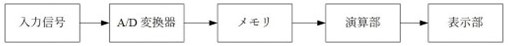
\includegraphics[width=.5\linewidth]{img/1.jpg}
  \caption{ディジタルオシロスコープの基本構成}
  \label{im1}
  \end{center}
\end{figure}

\mysubsection{ディジタルオシロスコープの動作原理について}
ディジタルオシロスコープは、観測信号(アナログ信号)をA/D変換によってディジタル信号に変換し、
そのデータをメモリに保存してから波形を表示する。ディジタル信号で画面に線を描画するためには、観測信号と掃引信号を同期する必要がある。
同期の取り方は、トリガ同期方式を用いる。トリガ同期方式は、測定したい波形の振幅よりも少し小さい振幅にトリガレベルを設定することによって、
入力信号の振幅がトリガレベルを超えたときに掃引信号が発生する方式である。
また、ディジタルオシロスコープにおいて、トリガレベルは自由に設定できる。

\mysubsection{AD変換器について}
アナログ信号をディジタル信号に変換することをA/D変換という。 
A/D変において、\textbf{\textgt{サンプリング (標本化)・量子化・符号化}} の操作を行う必要がある。
サンプリング (標本化)・量子化を図\ref{im2}に示す。

\begin{figure}[htb]
  \begin{center}
  \subfigure[サンプリング(標本化)]{
  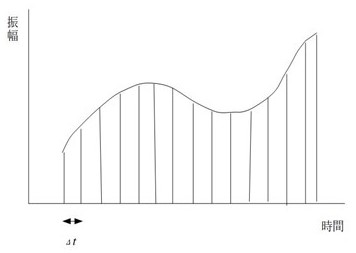
\includegraphics[width=.45\columnwidth]{img/2.jpg}
  }
  \subfigure[量子化]{
  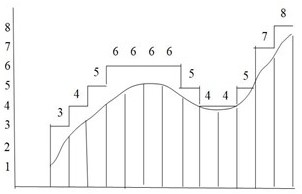
\includegraphics[width=.45\columnwidth]{img/3.jpg}
  }
  \caption{サンプリング・量子化について}
  \label{im2}
  \end{center}
\end{figure}

\begin{description}
  \setlength{\parskip}{0cm} % 段落間
  \setlength{\itemsep}{0cm} % 項目間
  \item[サンプリング] 時間的に連続な波形から時間間隔$\varDelta t$ごとに波形の振幅を取り出す操作のことである。
  $\varDelta t$を\textbf{\textgt{サンプリング間隔}}、その逆数を\textbf{\textgt{サンプリング周波数}}という。
  サンプリング定理によるとサンプリング周波数を元のアナログ信号に含まれている最大周波数の2倍以上にすれば、元の波形を再現することができる。
  \item[量子化] サンプリングした波形の振幅を分割して、最も近い整数を割り当てる操作のことである。
  量子化前後の誤差を\textbf{\textgt{量子化誤差}}といい、量子化に波形の分割数が少ないと、量子化誤差が大きくなる。
  \item[符号化] 量子化された整数(10進数)を2進数に変換する操作である。
\end{description}

\mysubsection{本実験で使用した表計算ソフトについて}
表計算を行う際、実際にデータを入力する一桝をセルという。
各セルに計算式を表す \verb|“=”|(イコール)の記号を先頭に入力し、
算術計算の式を入力することによってそのセルに、その演算結果を入力できる。

\mysubsection{フーリエ級数展開について}
周期関数$f(t)$ (周期$T$)を、
次の式のように三角関数の項と$b_0$の式で表すことができることを示す。
\begin{screen}
  \begin{equation}
    f(t) = b_0+\sum_{n = 1}^{\infty} b_n \cos n\omega t + \sum_{n = 1}^{\infty} a_n \sin n\omega t \label{eq1}
  \end{equation}
\end{screen}
  
式\eqref{eq1}の、$b_0$、$a_n$、$b_n$をフーリエ係数という。また、フーリエ係数は、それぞれ、式\eqref{eq2}~\eqref{eq4}のように表すことができる。

\begin{screen}  
  \begin{gather}
    b_0 = \frac{1}{T}\int_{0}^{T}f(t) \,dt \label{eq2} \\
    b_n = \frac{1}{T}\int_{0}^{T}f(t)\cos n\omega t \,dt \label{eq3} \\
    a_n = \frac{1}{T}\int_{0}^{T}f(t)\sin n\omega t \,dt \label{eq4}
  \end{gather}
\end{screen}

\mysubsection{数値積分について}
時間間隔が$\varDelta t$で標本化された関数$f_i = f(t_i) (i = 1, 2, 3, \dots N)$の定積分は、式\eqref{eq5}で近似できる。
数値積分で近似している部分を図\ref{im3}に長方形で示す。
\begin{screen} 
  \begin{equation}
    \int_{t_1}^{t_n}f(t) \,dt = \int_{t_n}^{t_{N-1}}f(t) \,dt + \varDelta t \sum_{i = 1}^{N-1}f_i \label{eq5}
  \end{equation}
\end{screen}

\begin{figure}[htbp]
  \begin{center}
  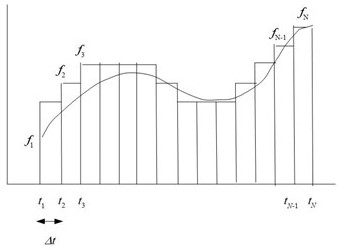
\includegraphics[width=.5\linewidth]{img/4.jpg}
  \caption{数値積分}
  \label{im3}
  \end{center}
\end{figure}
\mysection{実験方法}
本実験で使用する器具を表\ref{tb1}に示す。

\begin{table}[ht]
  \centering
  \caption{使用器具}
  \begin{tabular}[t]{lcc}
  \toprule
  \multicolumn{1}{c}{使用機器}&\multicolumn{1}{c}{型番}&規格等\\
  \midrule
  ディジタルオシロスコープ&Tektronix&TDS2012B, 100-240 V, 100 MHz\\
  ファンクションジェネレータ&IWATSU&SG-4105, 110-240 V, 10-15 MHz\\
  パーソナルコンピュータ&HP&--\\
  表計算ソフト&Microsoft Excel&--\\
  \bottomrule
  \end{tabular}
  \label{tb1}
\end{table}

\begin{enumerate}
  \setlength{\parskip}{0cm} % 段落間
  \setlength{\itemsep}{0cm} % 項目間
  \item ファンクションジェネレータの出力を振幅1 V周波数100 kHz、デューティファクター 20\verb|%| の方形波に設定する。
  \item ディジタルオシロスコープのDCモードのACモードの画面の出力の違いを確認する。
  \item ファンクションジェネレータの出力を振幅50 mV、周波数100.1 kHzの正弦波に設定する。
  \item ディジタルオシロスコープの掃引モードをオートモードとして、トリガレベルを操作し、正・負のピーク値の間にある場合・ない場合それぞれの違いを観測する。
  \item 掃引モードをノーマルに変更し、トリガレベルを上記 (4) と同様に操作し、波形を観測する。
  \item ディジタルオシロスコープの波形取り込みモードをサンプルからアベレージに変えて、波形の変化を観測する。
  \item 水平軸間隔を2.5 ms ~ 5 msとしたときの表示波形の周波数を測定する。
  \item ディジタルオシロスコープで観測した波形のデータをUSBメモリに保存する。
  \item ファンクションジェネレータの出力を振幅1 V周波数10 kHzの三角波に設定する。
  \item 上記 (9)のデータを保存し、サンプリング間隔と量子化間隔を求める。
  \item ファンクションジェネレータの出力を振幅220 mV周波数1600 Hz、デューティファクター 66 \verb|%| の方形波の波形データを保存する。
  \item 上記 (11) で保存した波形を、 PCの表計算ソフトで読み込み、各セルで、
  式\eqref{eq5}の算術演算を行い、フーリエ係数 $b_0, b_1, b_2, b_3, b_4, b_5, b_6, a_1, a_2, a_3, a_4, a_5, a_6$ を求める。
  \item 上記 (12) で求めたフーリエ係数を用いて、観測波形の近似波形を作る。
  \item 上記 (7) で保存した波形を保存波形の図から読み取り、式\eqref{eq6}で近似する。\\
  \begin{screen}
  \begin{equation}
    f(t) = \left\{
    \begin{array}{ll}
    V_1 \si{[\milli V]} & (t_1 \leqq t < t_2)\\
    V_2 \si{[\milli V]} & (t_2 \leqq t < t_3)\\
    \end{array}
  \right.
  \label{eq6}
  \end{equation}
\end{screen}
  \item フーリエ係数の定義の式から手計算し、式\ref{eq5}の計算結果と比べる。
\end{enumerate}


\mysection{結果}
\subsection{実験1}
実験 (2) の結果について、 DCモードの波形と比べてACモードの波形が全体的に画面の縦軸方向に移動した。
実験 (4) の結果について、トリガレベルが測定波形の正・負のピーク値の間にある時、波形が表示され、トリガレベルを負から正の値に動かすと、波形が全体的に横軸方向に動き、逆にトリガレベルを正から負の値に動かすと波形が全体的に横軸の逆方向に動いた。また、波形の外にトリガレベルを動かすと、波形が横軸方向に揺れ動いて表示された。
実験 (5) の結果について、正・負のピーク値の間にトリガレベルがあるとき、波形が表示され、トリガレベルを負から正、正から負に動かした場合の表示波形の変化は上記 (2) の結果に等しい。しかし、波形の外にトリガレベルを動かすと表示画面上方に小さく “ Ready ” の文字が表示され、波形の線が薄くなった。また、薄くなった線はファンクションジェネレータの電源をOFFにしても消えなかった。
実験 (6) の結果について、ディジタルオシロスコープの波形取り込みモードがサンプルのときと比べて、アベレージモードに変えると、波形の線が細くなった。
実験 (7) の結果について、 50 msの区間において5周期分の波形が観測されたため、\\
  \begin{equation*}
    \frac{5}{5.0\times10^{-2}} = 100 \si{[Hz]}
  \end{equation*}
よって、100 \si{[Hz]}である。
実験 (10) の結果について、サンプリング間隔を求めるために用いたデータを表\ref{tb2}に示す。
  \begin{table}[ht]
    \centering
    \caption{サンプリング間隔を求めるために用いたデータ (抜粋)}
    \begin{tabular}[t]{rr}
    \toprule
    \multicolumn{1}{c}{経過時間 \textit{t} \si{[s]}}&\multicolumn{1}{c}{オシロスコープの出力電圧 \si{[V]}}\\
    \midrule
    0&0.224\\
    0.000001&0.224\\
    0.000002&0.224\\
    0.000003&0.224\\
    0.000004&0.224\\
    0.000005&0.224\\
    0.000006&0.224\\
    0.000007&0.224\\
    0.000008&0.224\\
    0.000009&0.224\\
    \bottomrule
    \end{tabular}
    \label{tb2}
  \end{table}

  表\ref{tb2}において、サンプリング間隔が左の列が時間間隔を表すデータの、連続する上下のデータ同士の間隔であるため、その間隔は、\textbf{0.0000001} \si{[s]}である。
また、量子化間隔は右の列の連続する上下のデータ同士の間隔であるため、その間隔は、\textbf{20} \si{[mV]}である。
なお、この波形を観測したとき、\textbf{\textgt{水平軸レンジ}}: \textbf{0.000025} \si{[s]}、 \textbf{\textgt{垂直レンジ}}: \textbf{500} \si{[mV]}であった。

\mysubsection{実験2}

  数値積分の計算結果の有効数字について、式\eqref{eq5}の計算において、標本化された関数の和と時間間隔との積で、標本化された関数の末位は小数第3位であるため、標本化された関数の和は、最小桁を小数第3位とする。
  次に、標本化された関数の和と時間間隔との積について、関数の和の位取りは3桁で、時間間隔の位取りは7桁であるため、積の誤差を考慮し、意味のある数字のみを残すため、位取りの少ない方に有効桁を合わせるので、式\eqref{eq5}の計算結果の有効数字を3桁とする。表\ref{tb3}, \ref{tb4}に実験 (12) の結果を示す。(単位\si{V})
  
  \begin{table}[h]
    \begin{center}
      \begin{tabular}{cc}
        \begin{minipage}{0.45\textwidth}
          \centering
          \caption{フーリエ級数$b_n$について}
          \begin{tabular}[t]{rr}
            \toprule
            \multicolumn{1}{c}{$b_n$}&\multicolumn{1}{c}{フーリエ級数の値 \si{[V]}}\\
            \midrule
            $b_0$&0.0712\\
            $b_1$&-0.117\\
            $b_2$&0.0641\\
            $b_3$&-0.00722\\
            $b_4$&-0.0261\\
            $b_5$&0.0270\\
            $b_6$&-0.007\\
            \bottomrule
          \end{tabular}
          \label{tb3}
        \end{minipage}
        \begin{minipage}{0.4\textwidth}
          \centering
          \caption{フーリエ級数$a_n$について}
          \begin{tabular}[t]{rr}
            \toprule
            \multicolumn{1}{c}{$a_n$}&\multicolumn{1}{c}{フーリエ級数の値 \si{[V]}}\\
            \midrule
            $a_1$&0.217\\
            $a_2$&0.0988\\
            $a_3$&0.000504\\
            $a_4$&0.0586\\
            $a_5$&0.0353\\
            $a_6$&0.00114\\
            \bottomrule
          \end{tabular}
          \label{tb4}
        \end{minipage}
      \end{tabular}
    \end{center}
\end{table}

実験 (13) の結果について、近似波形、$b_0$に関する波形、被測定波形を図\ref{im5} \verb|~| 図\ref{im6} に示す。(図\ref{im6}は$n = 6$におけるフーリエ級数展開を式\ref{eq2} \verb|~| \ref{eq4} に適用。)

\begin{figure}[H]
  \begin{center}
    \subfigure[フーリエ級数による近似 ($n = 3$まで)]{
      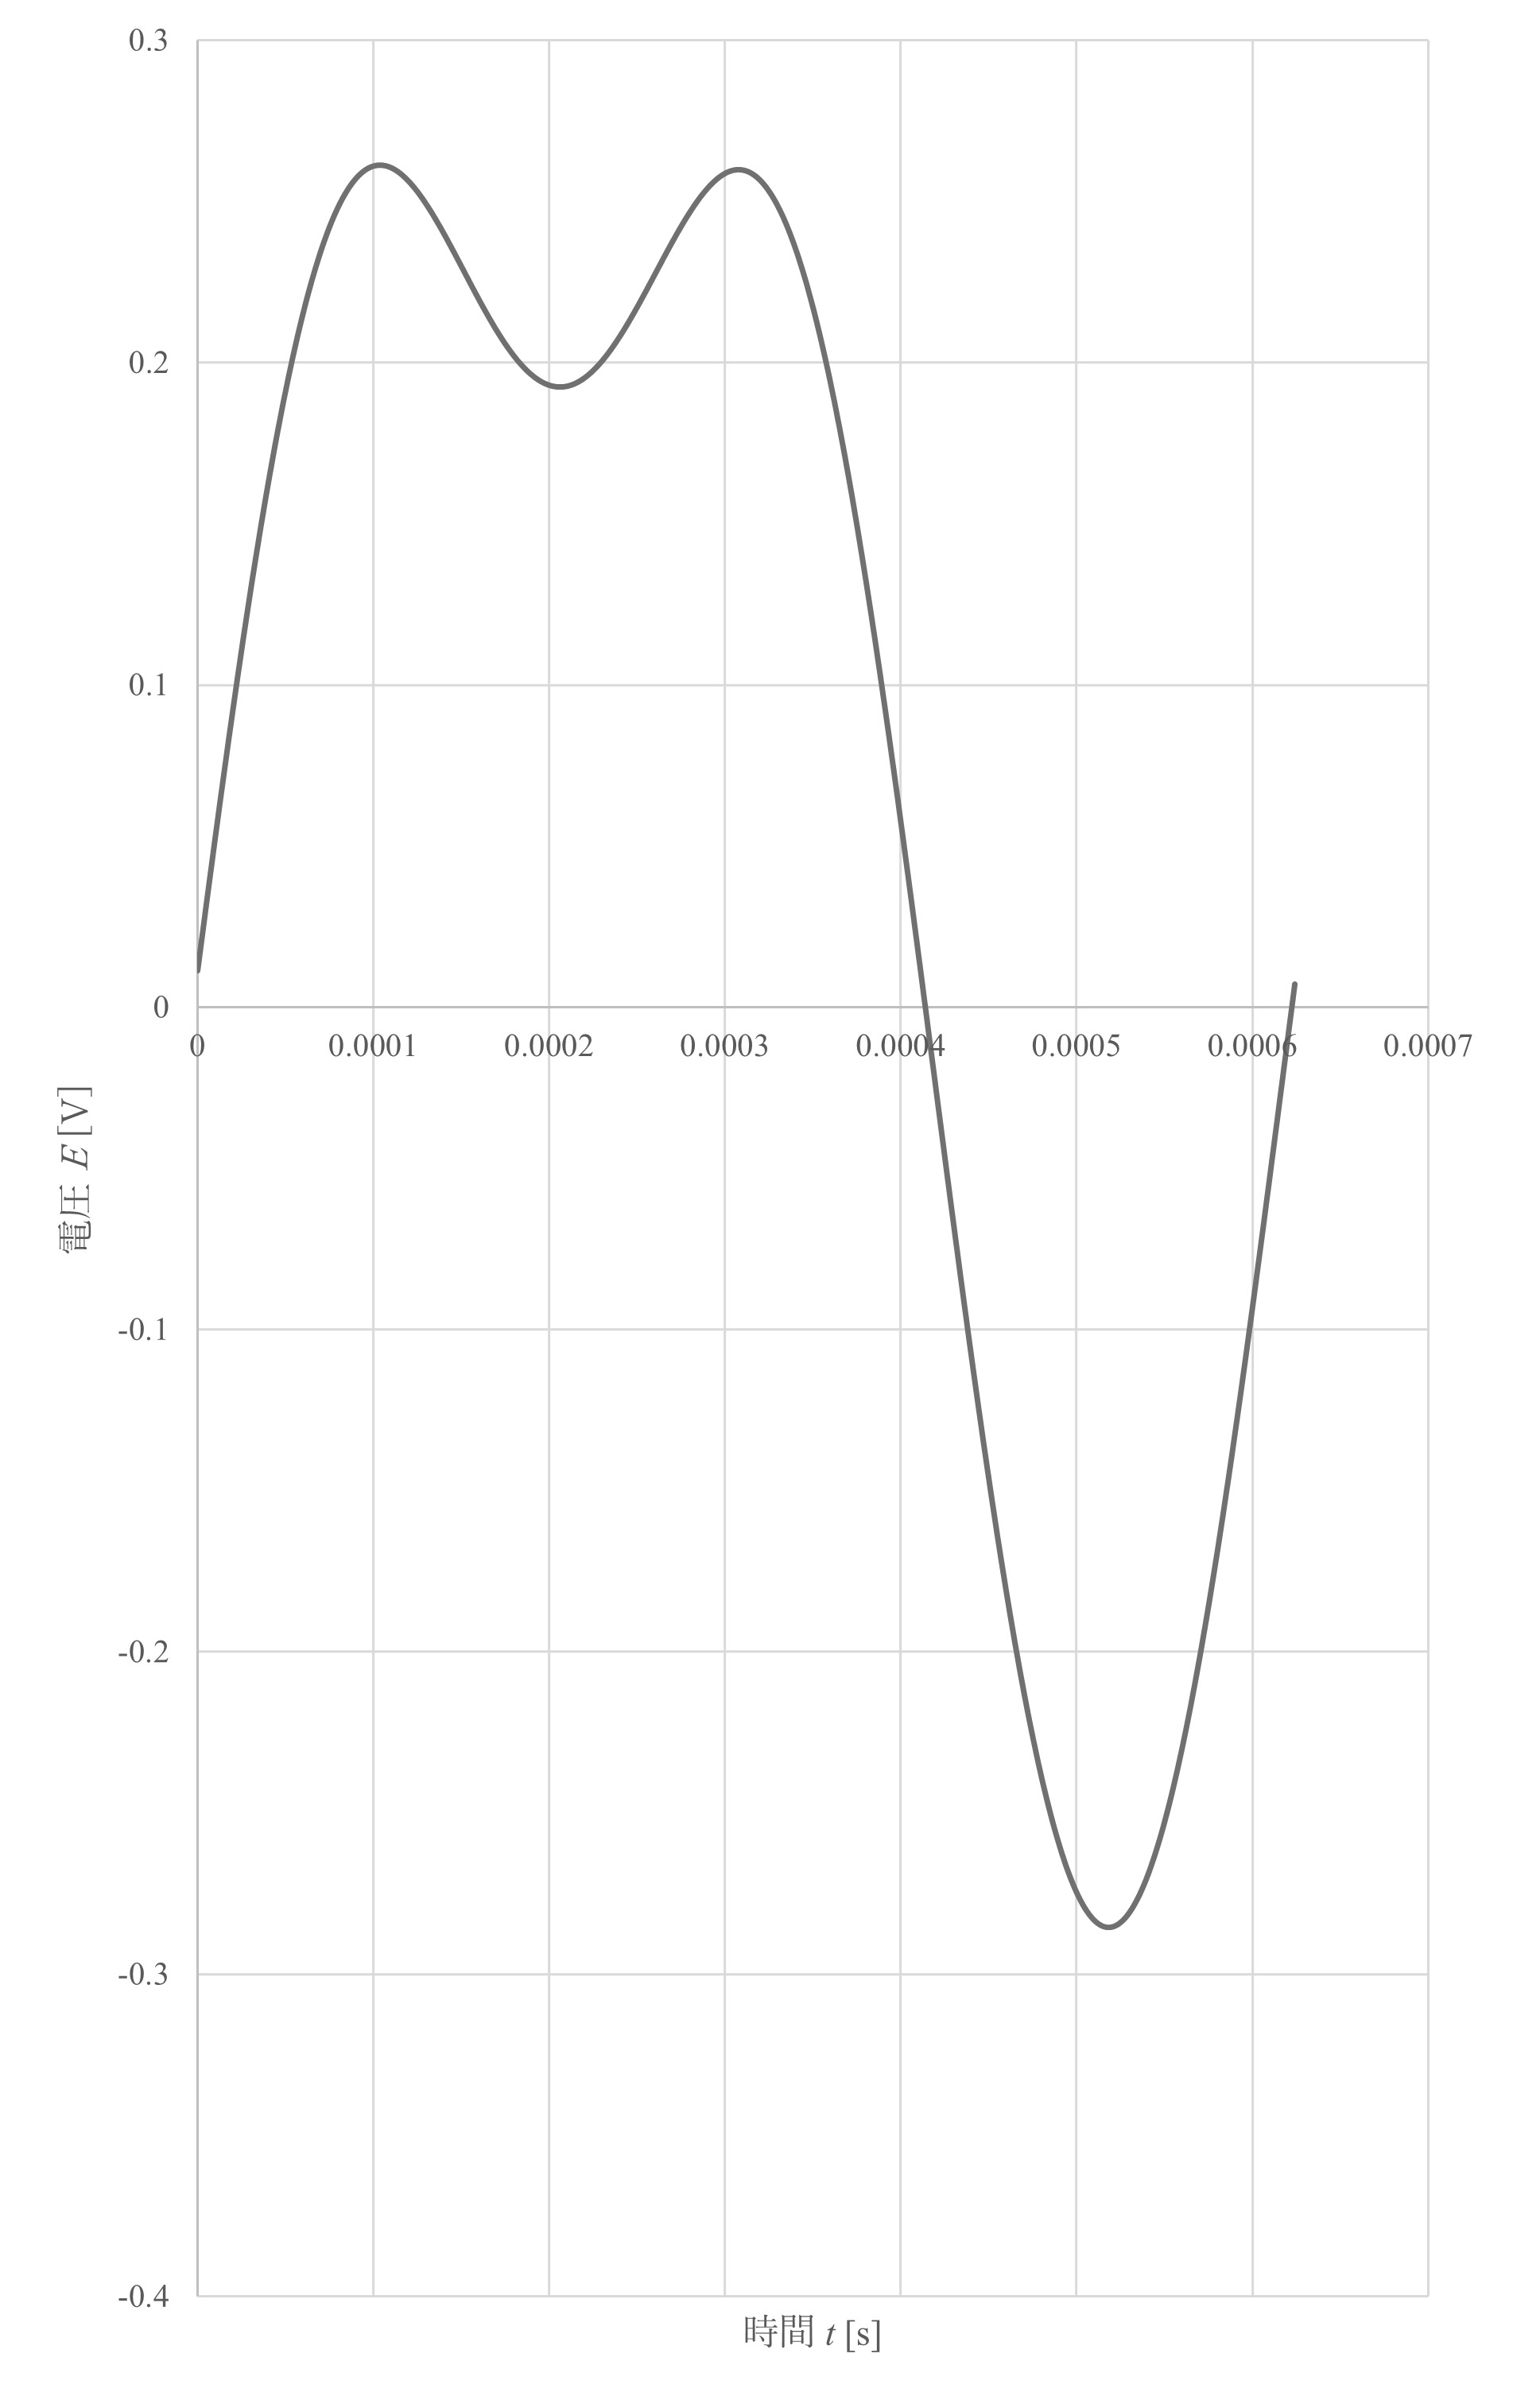
\includegraphics[width=.4\columnwidth]{img/5.jpg}
      \label{sub1}
    }~
    \subfigure[フーリエ級数による近似 ($n = 4$まで)]{
    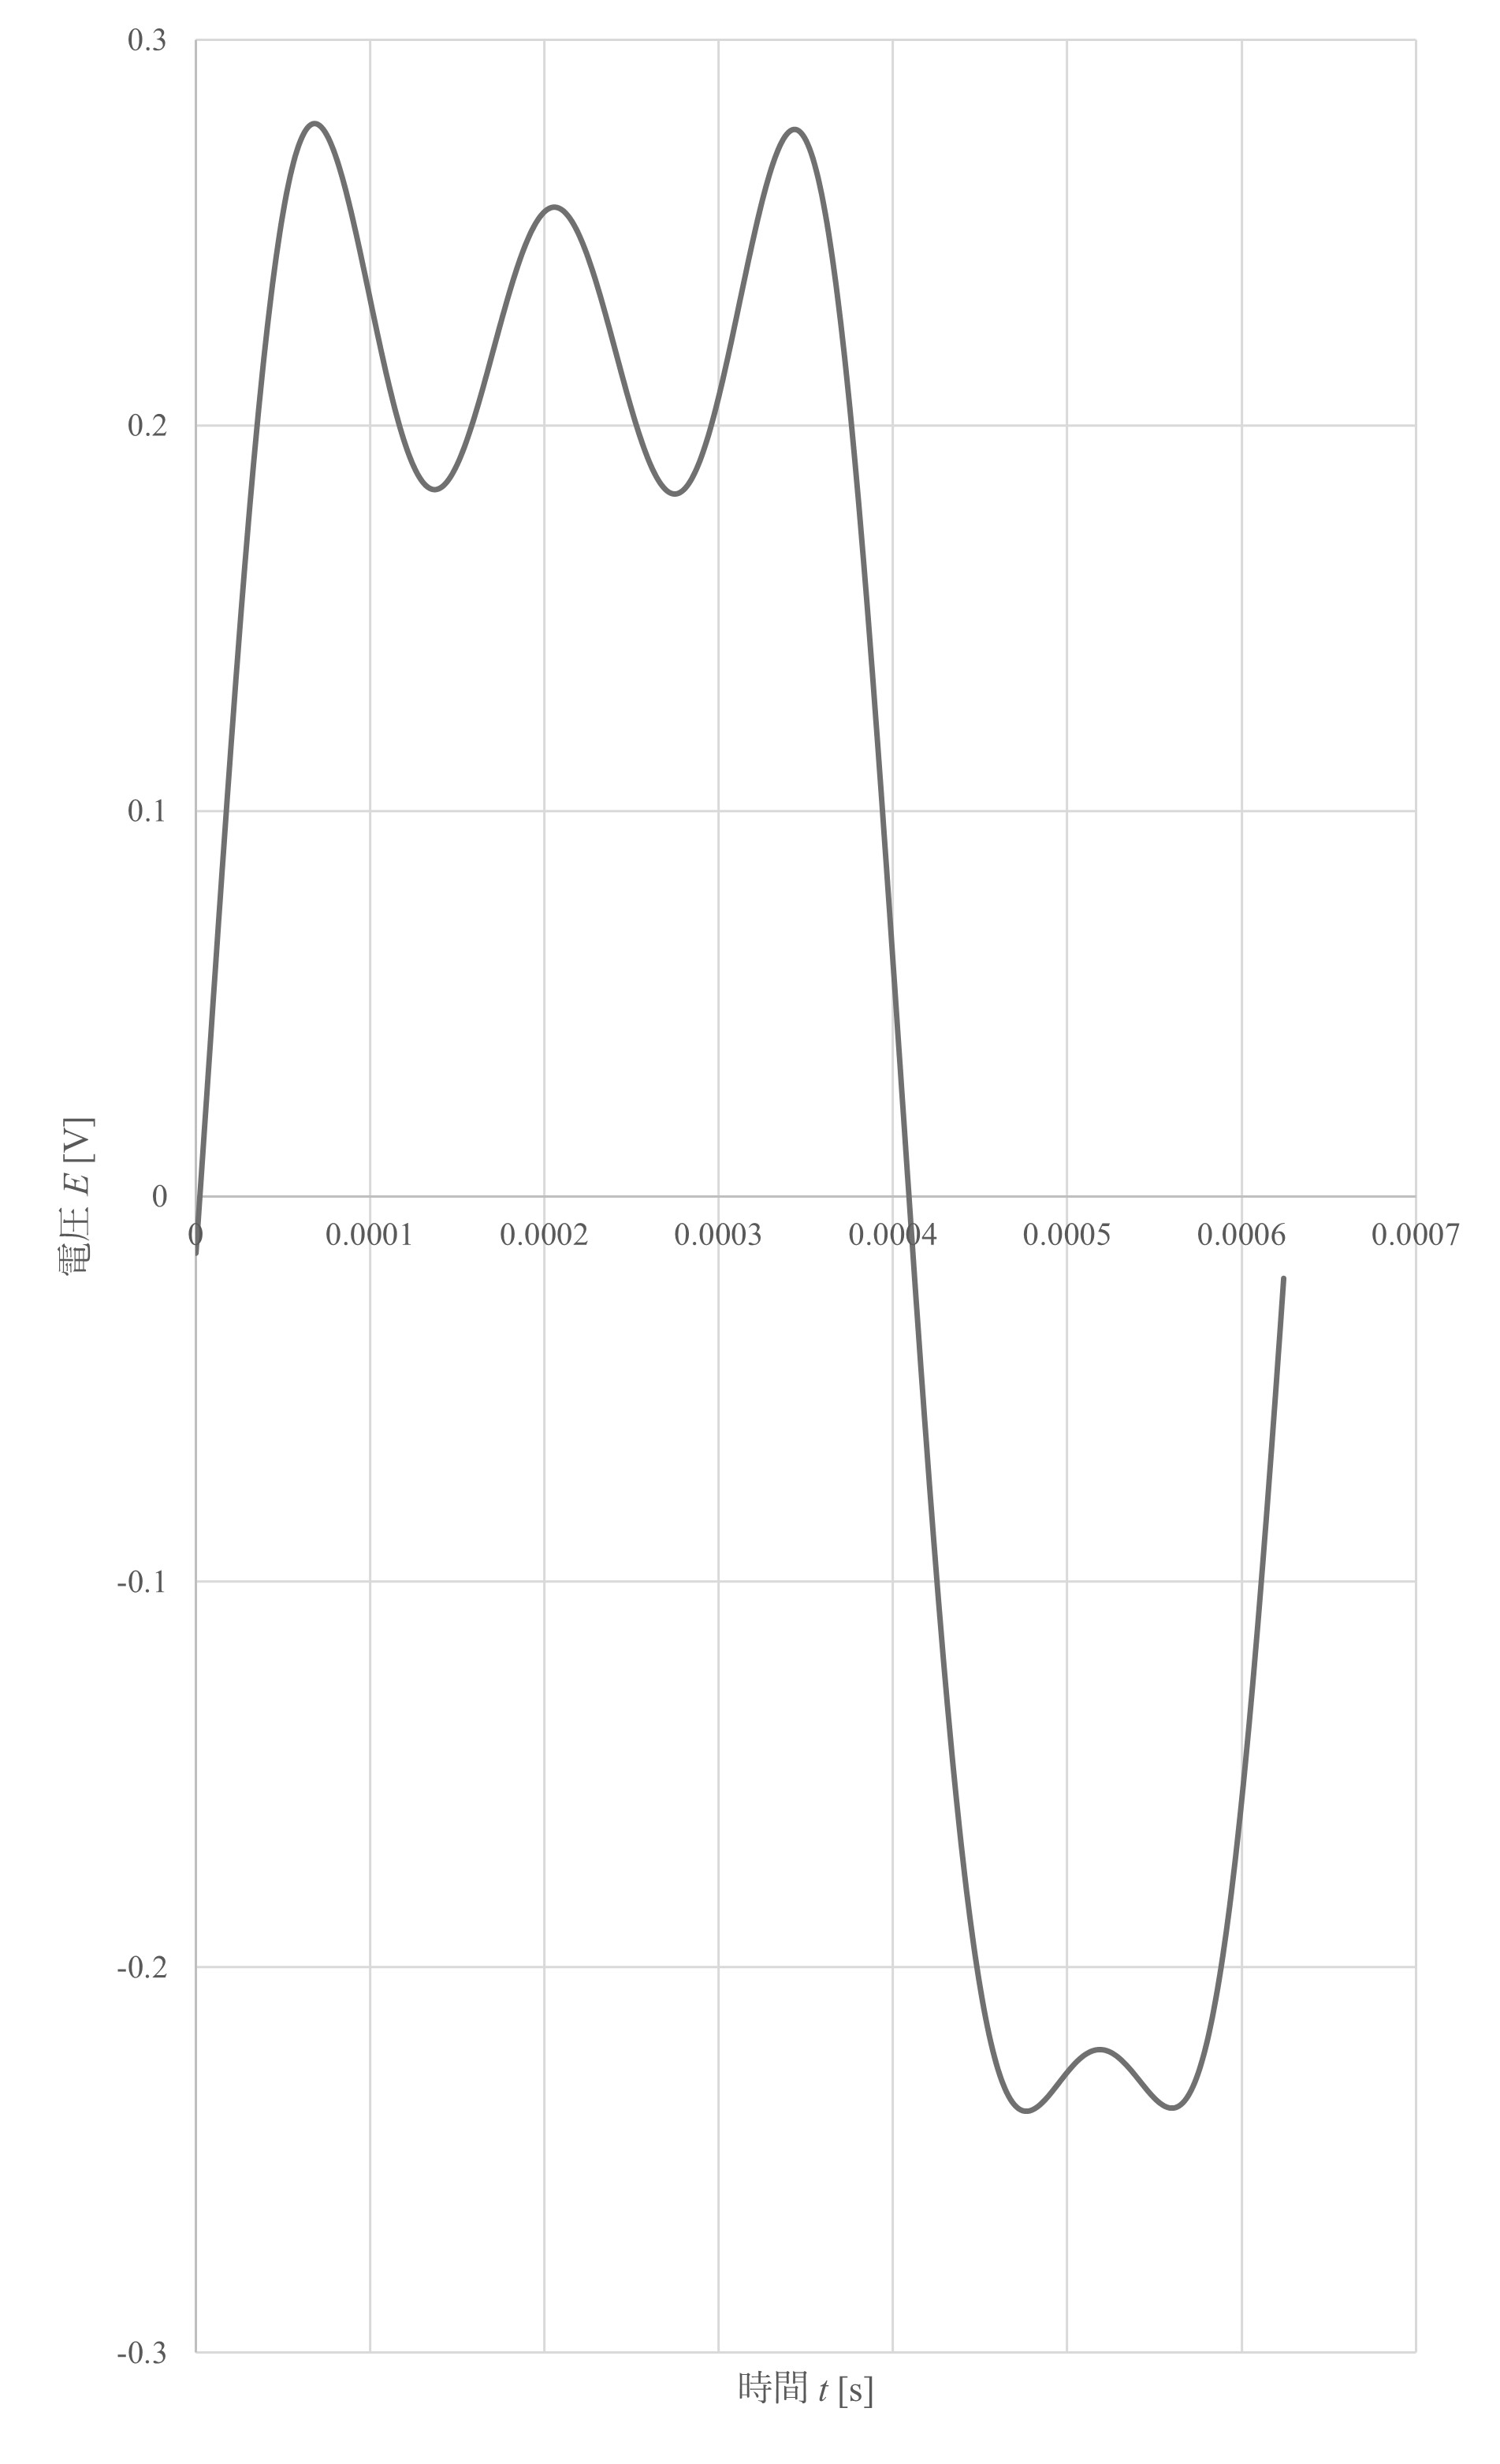
\includegraphics[width=.4\columnwidth]{img/6.jpg}
      \label{sub2}
    }
    \subfigure[フーリエ級数による近似 ($n = 5$まで)]{
    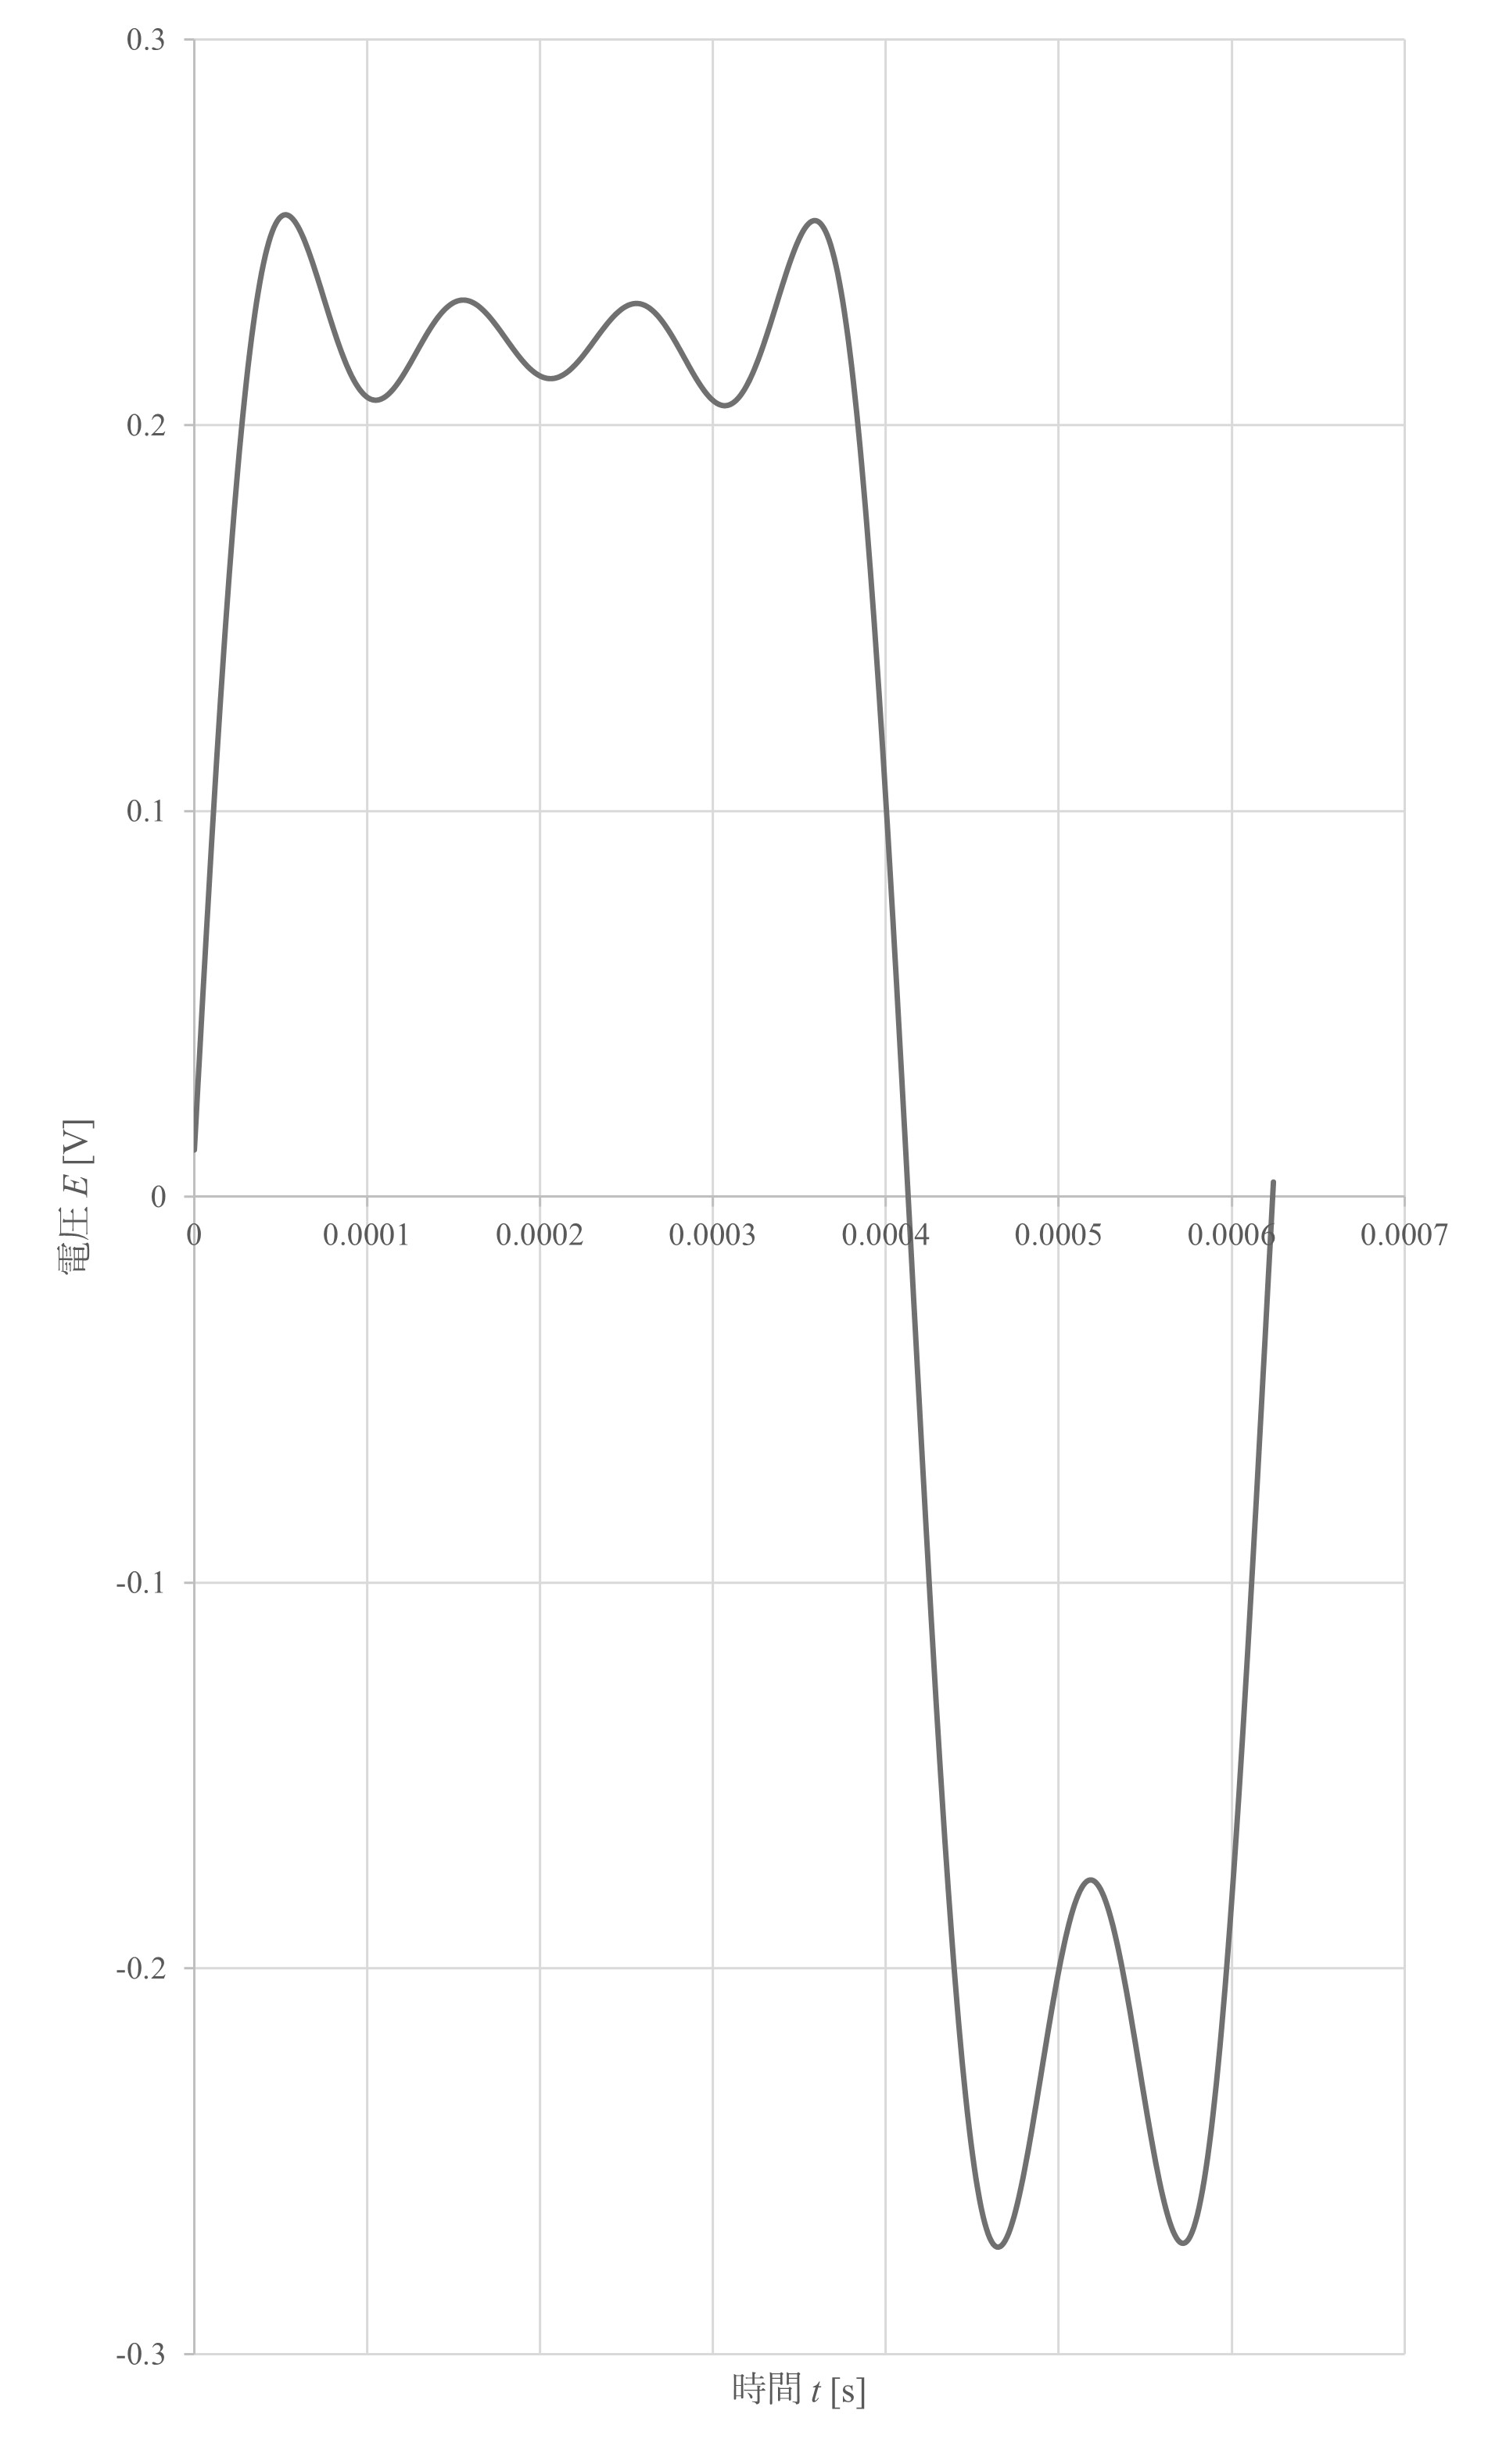
\includegraphics[width=.4\columnwidth]{img/7.jpg}
      \label{sub3}
    }~
    \subfigure[フーリエ級数による近似 ($n = 6$まで)]{
    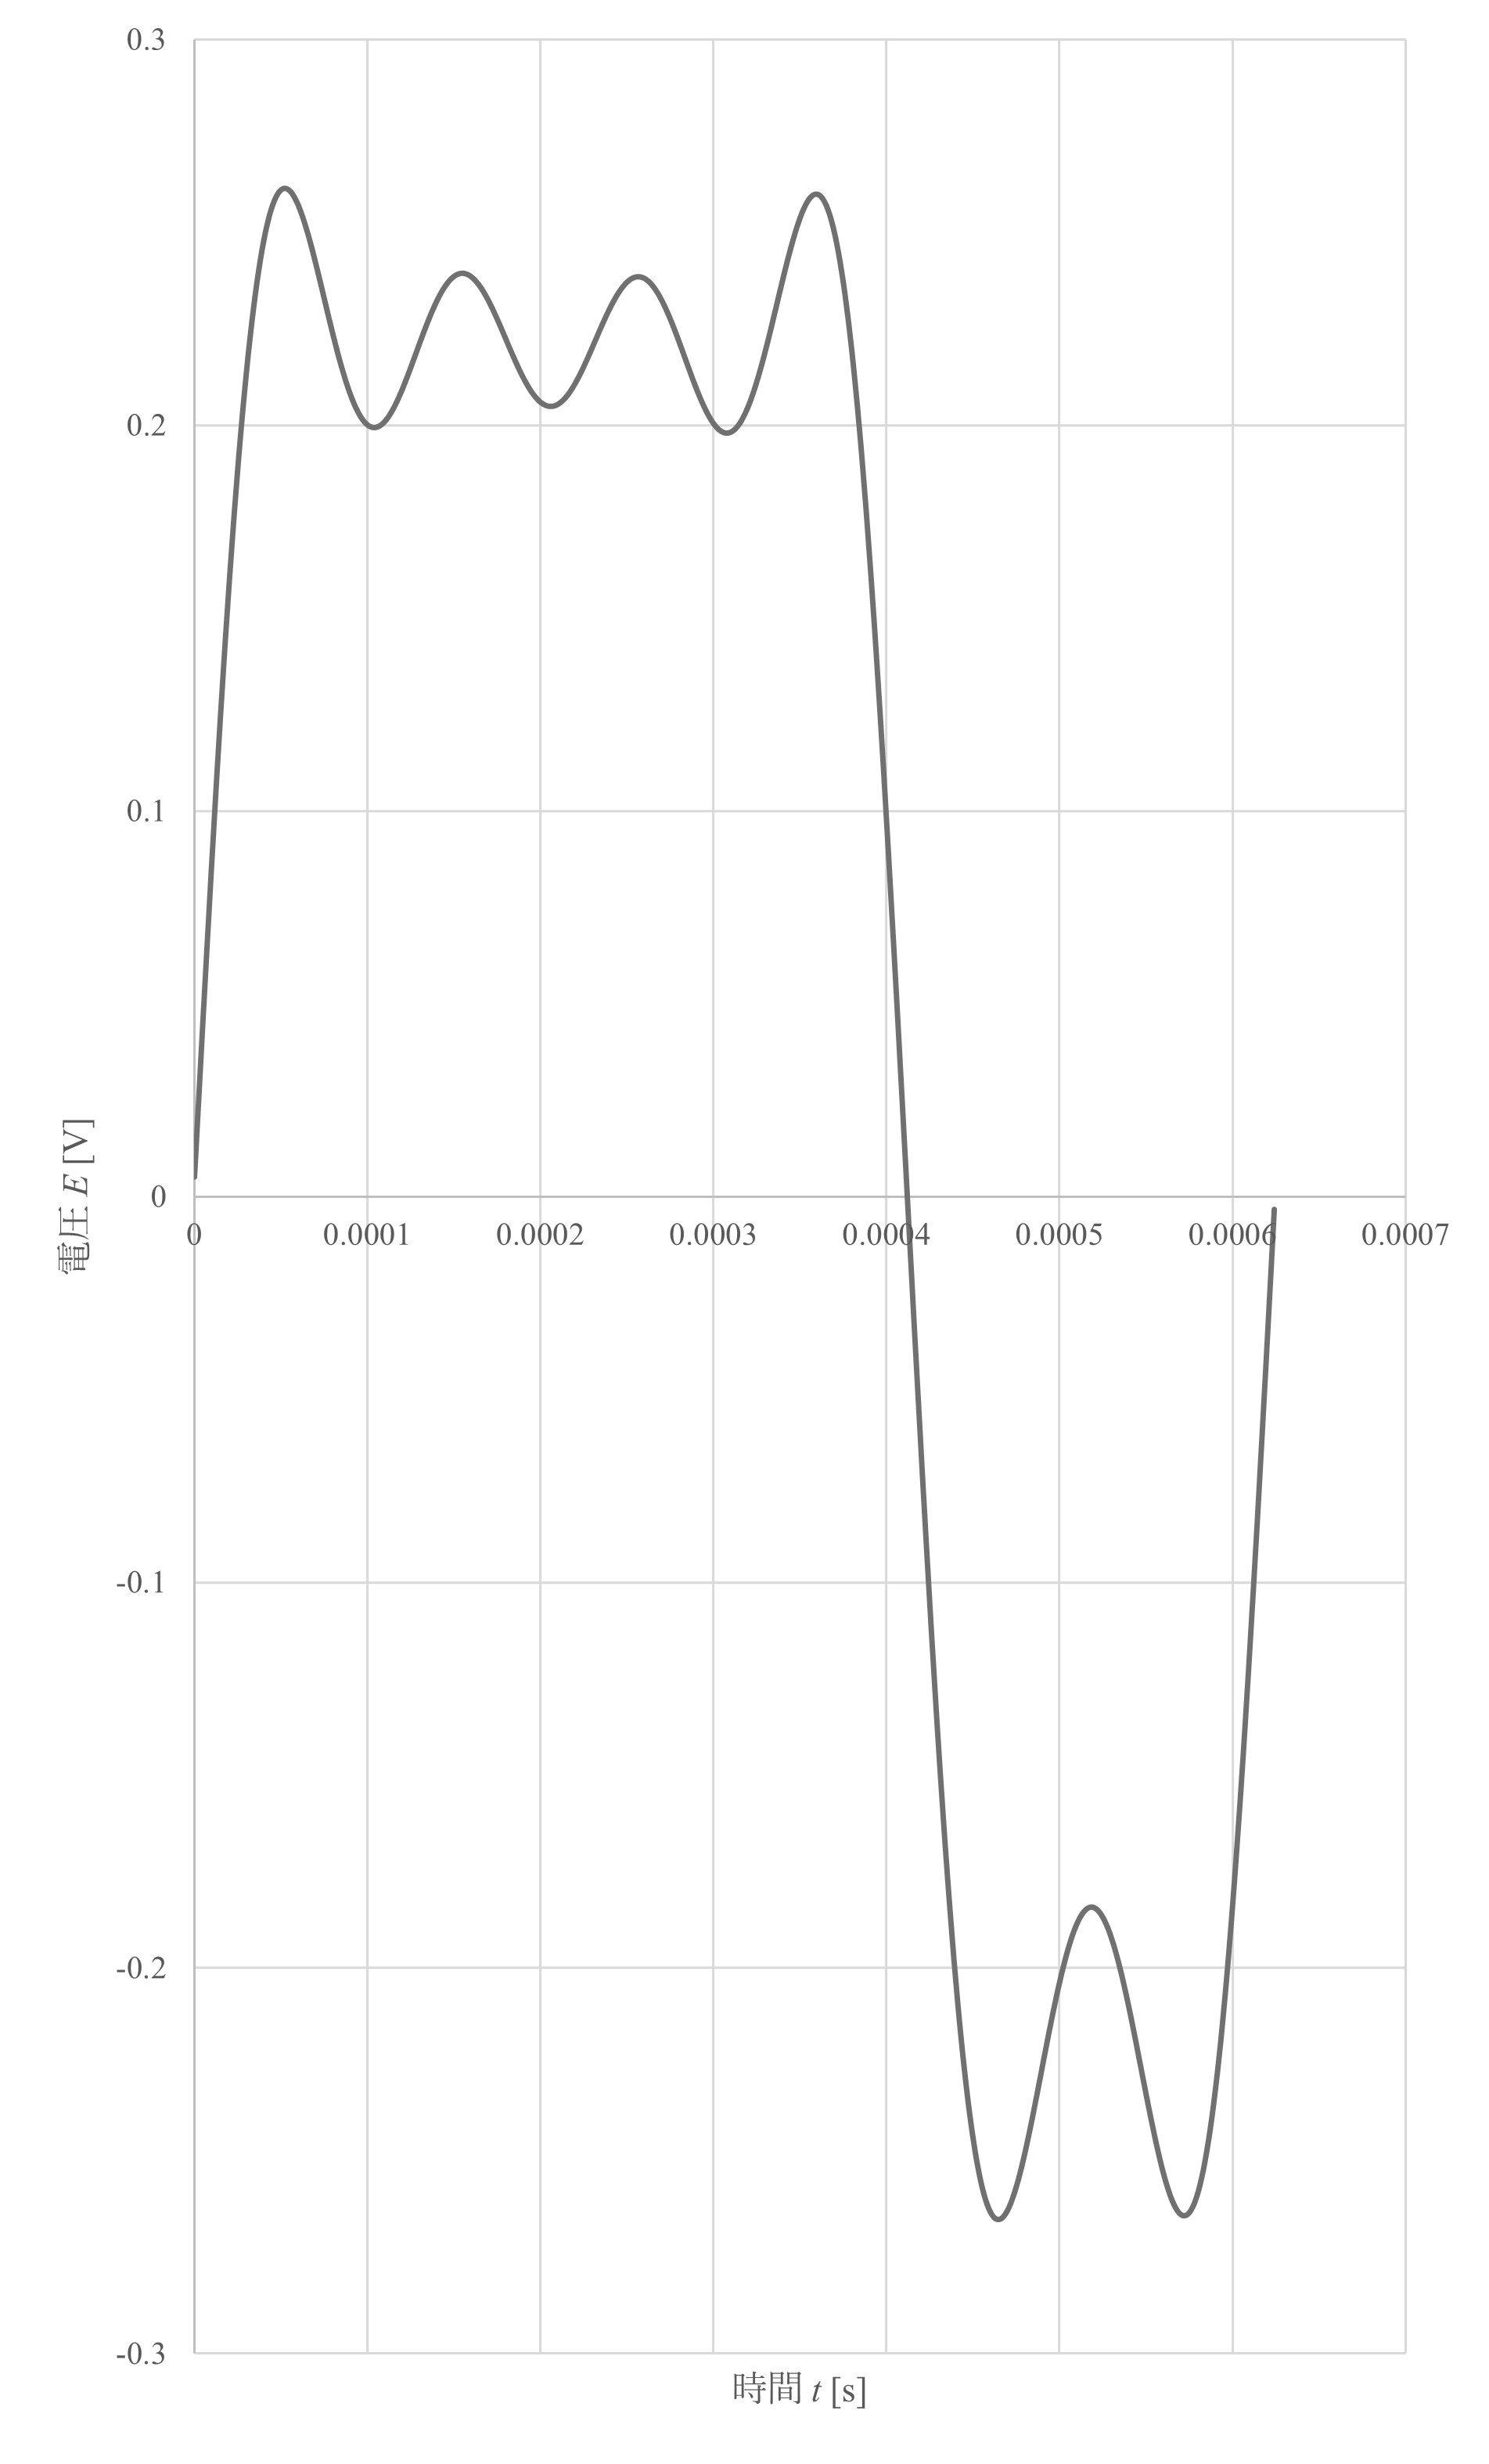
\includegraphics[width=.4\columnwidth]{img/8.jpg}
      \label{sub4}
    }
   \caption{フーリエ級数による近似}
   \label{im5}
   \end{center}
\end{figure}

\begin{figure}[H]
  \begin{center}
    \subfigure[$b_0$を足さずに計算した近似値($n = 6$まで)]{
      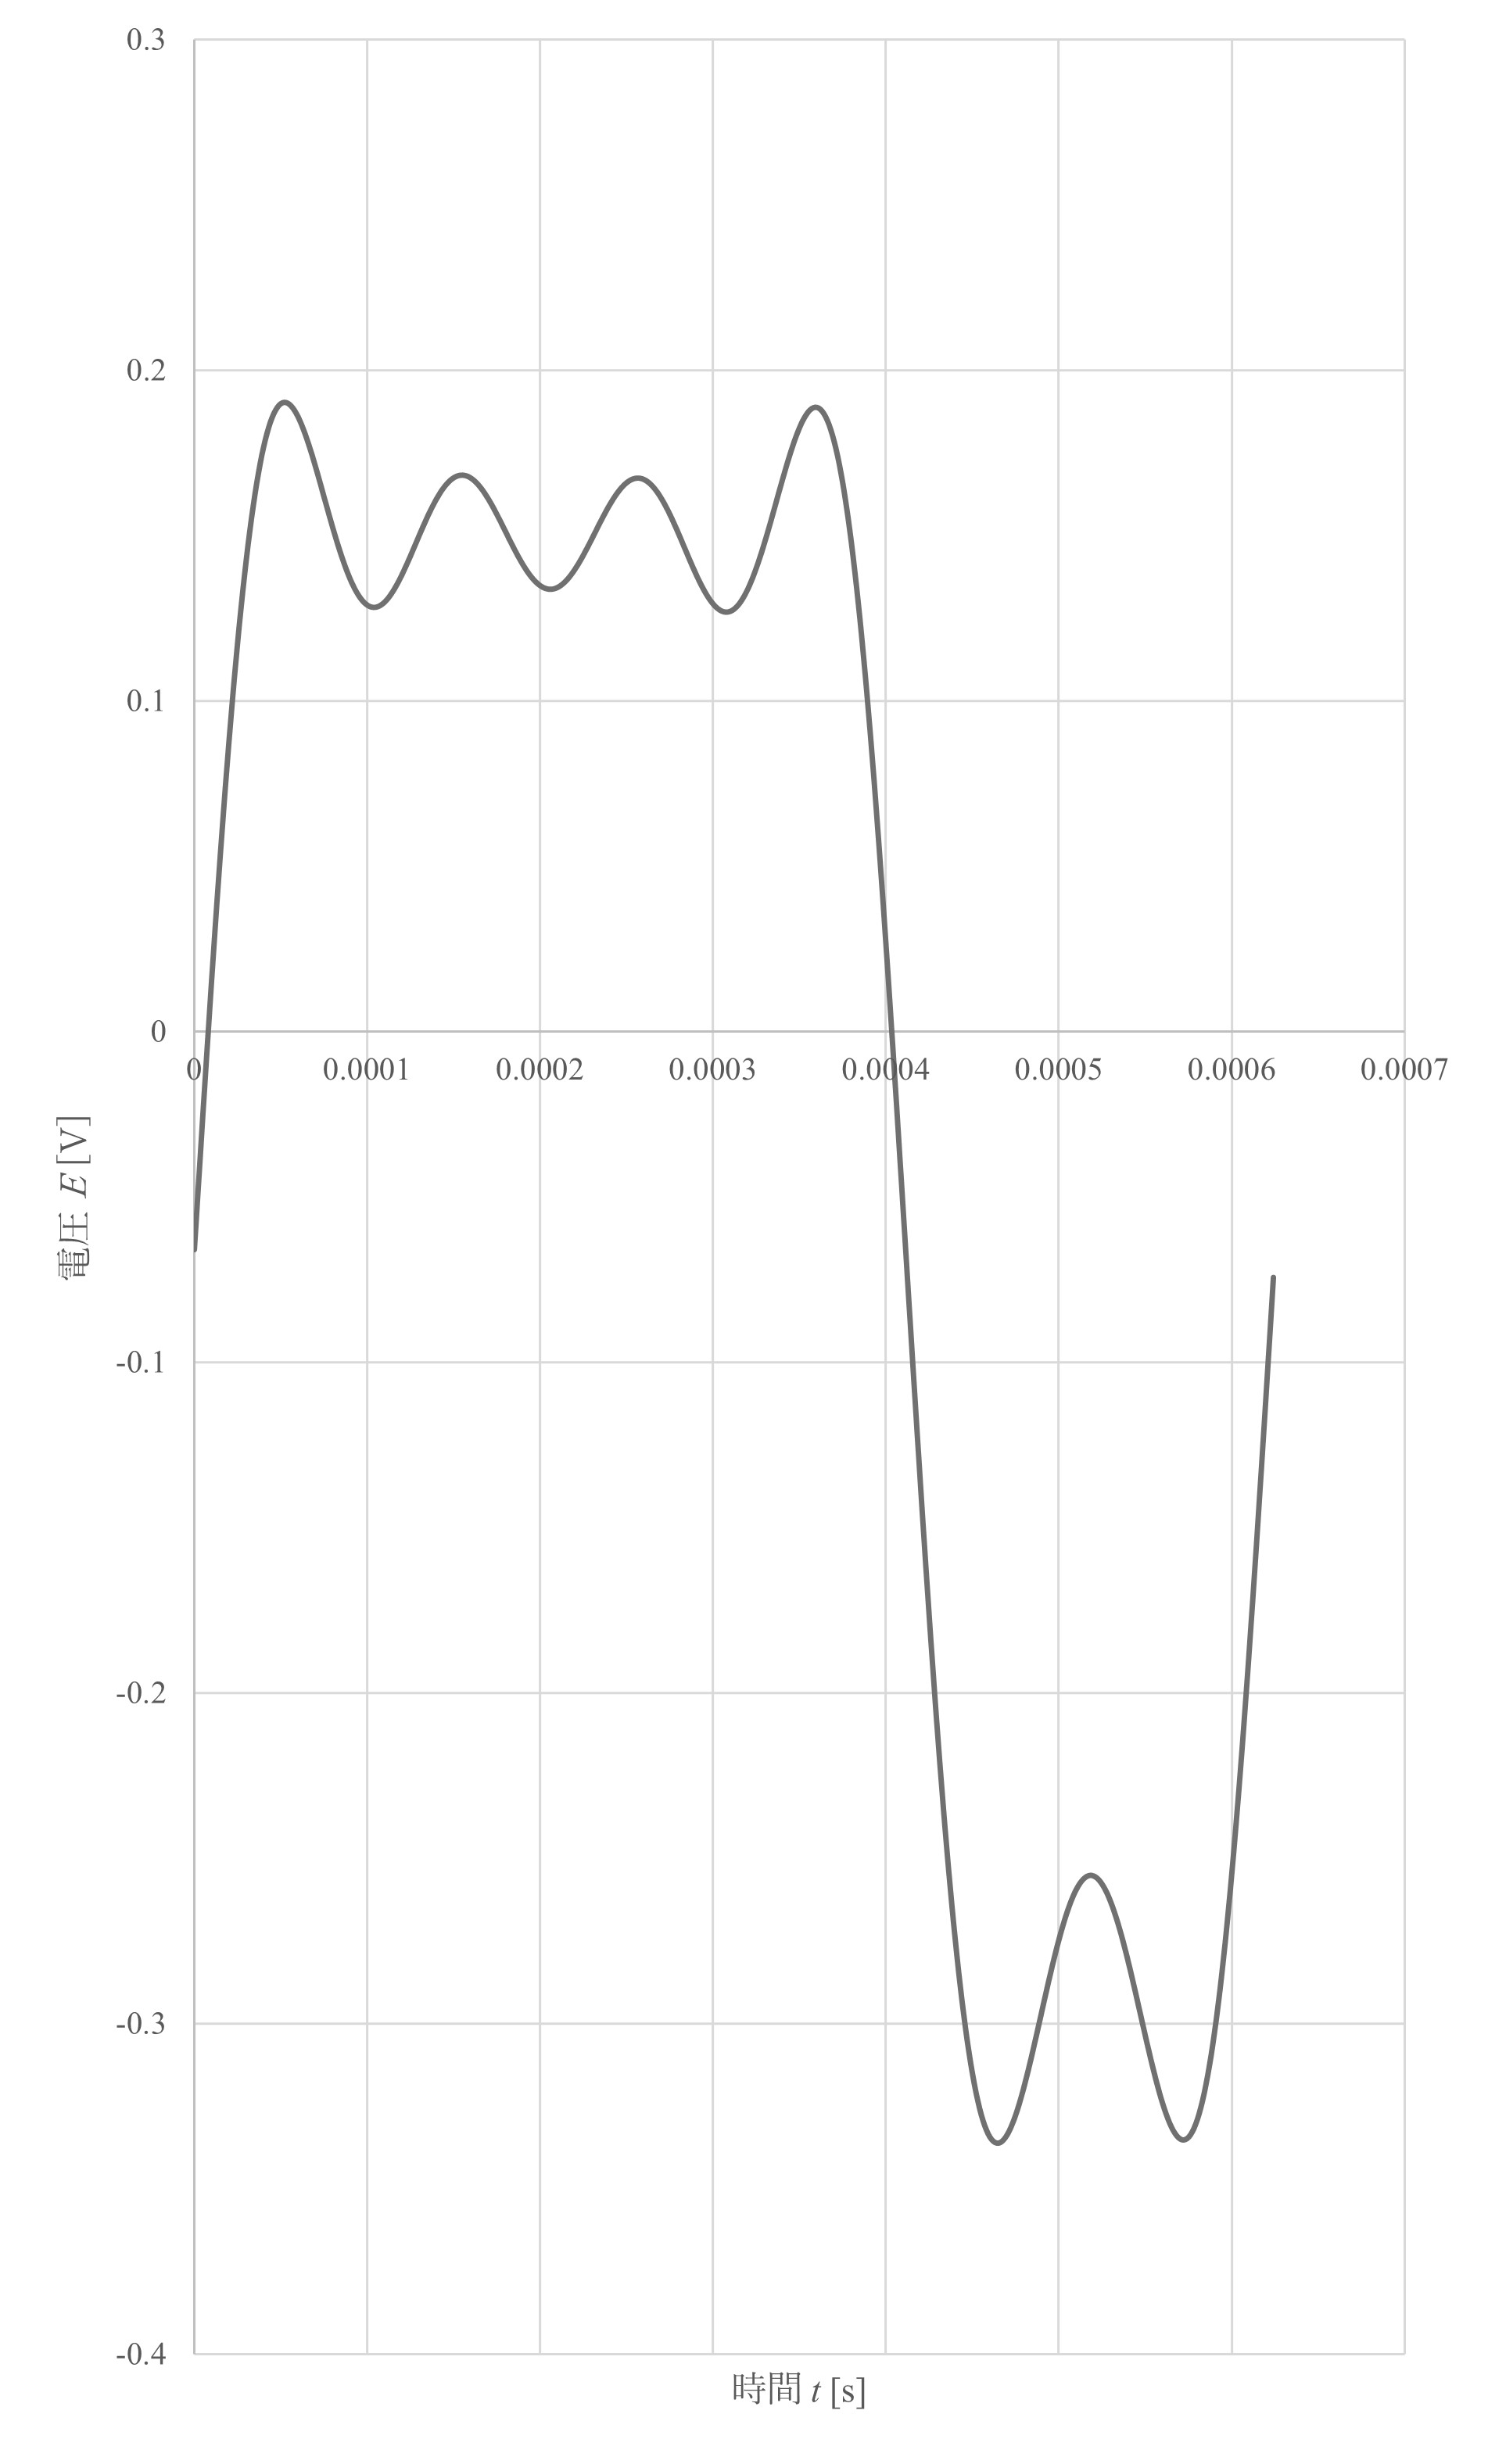
\includegraphics[width=.4\columnwidth]{img/9.jpg}
      \label{sub5}
    }
    \subfigure[被測定波形]{
    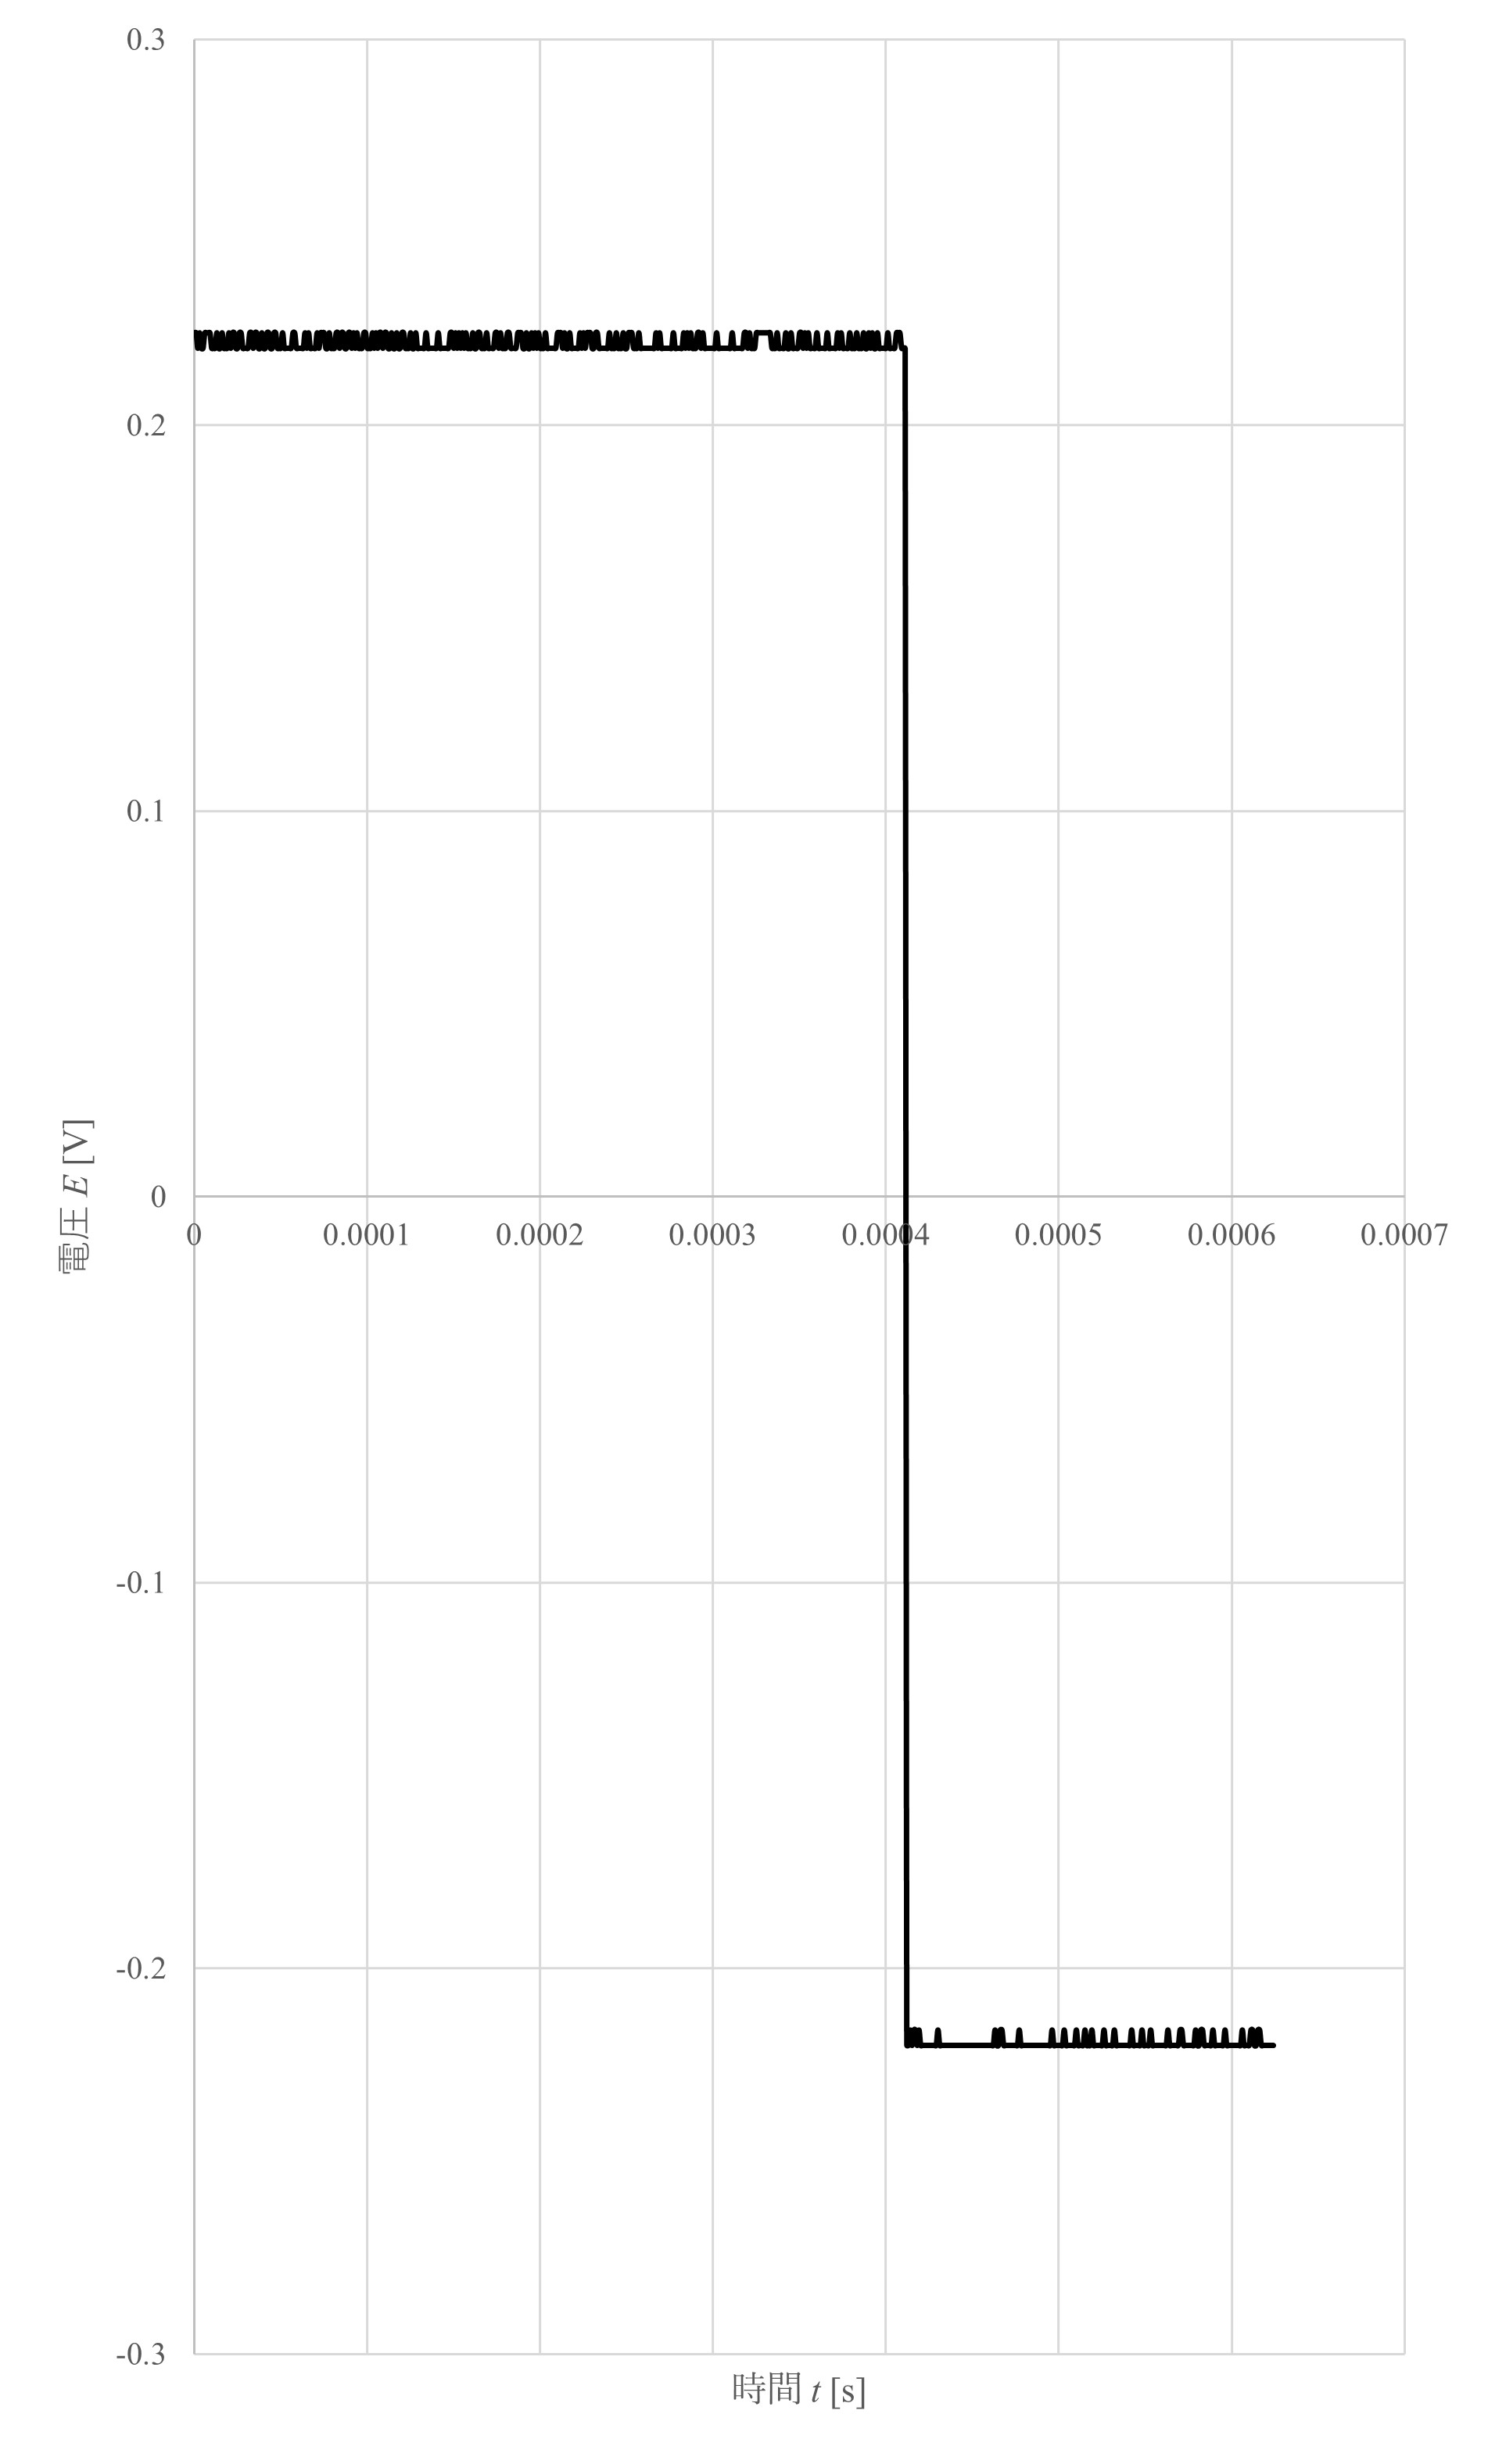
\includegraphics[width=.4\columnwidth]{img/10.jpg}
      \label{sub6}
    }~
    \subfigure[フーリエ級数展開の定義式による波形近似($n = 6$まで)]{
    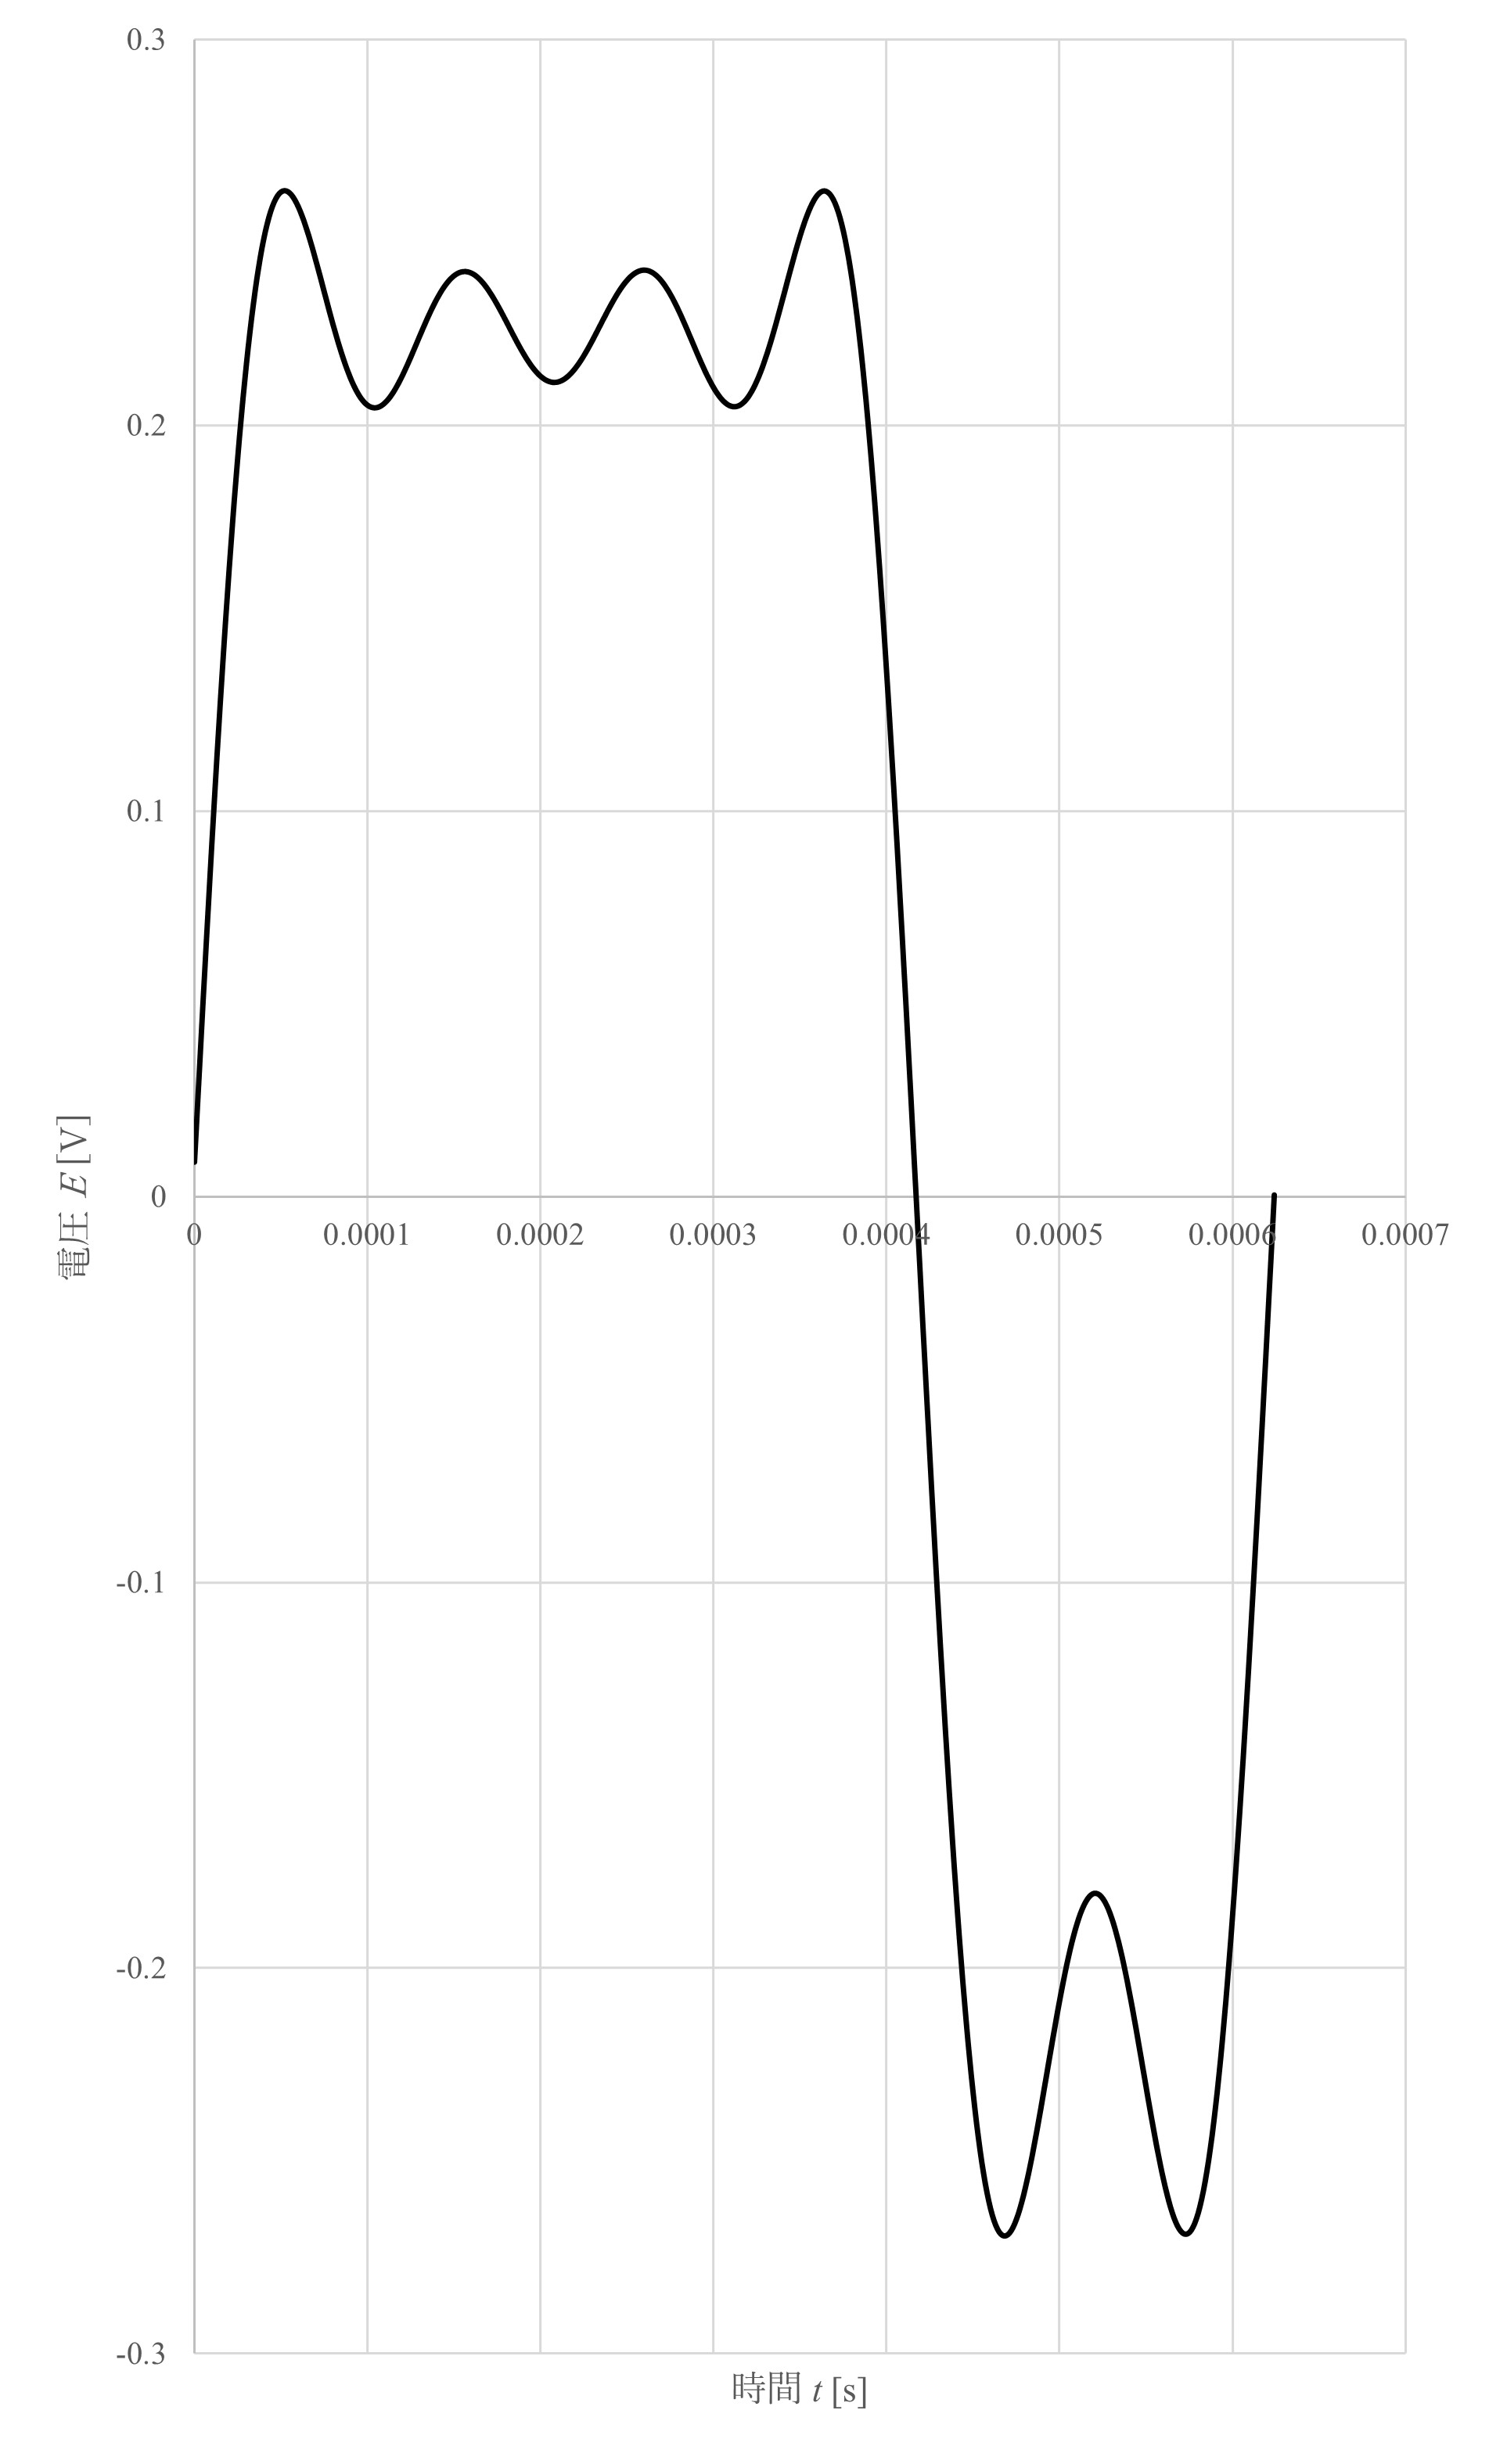
\includegraphics[width=.4\columnwidth]{img/11.jpg}
      \label{sub7}
    }
   \caption{フーリエ級数による近似}
   \label{im6}
   \end{center}
\end{figure}

実験 (14) の結果について、図\ref{im6} \subref{sub6}より、
\begin{screen}
  \begin{equation}
    f(t) = \left\{
      \begin{array}{ll}
        225 \si{[\milli V]} & (0 \leqq t < t \si{[s]})\\
        -220 \si{[\milli V]} & (0.000416 \leqq t < 0.000625 \si{[s]})\\
      \end{array}
      \right.
      \label{eq7}
    \end{equation}
\end{screen}

実験 (15) の結果について式\ref{eq2} \verb|~| \ref{eq4} によってフーリエ係数を計算した過程と結果を、
式\ref{eq9} ~ 式\ref{eq20}表\ref{tb5}, \ref{tb6} に示す。
フーリエ級数展開の有効数字について、式\ref{eq3}, \ref{eq4} の計算は、時間関数と三角関数の積で、時間関数の位取りは3桁で三角関数の位取りは9桁となっているから、
積において位取りの少ない方に有効桁を合わせるため、有効桁を3桁とする。
(角度はラジアンで計算、周期$T = 1/1600 \si{[s]} $)

\begin{screen}
\begin{equation}
  \begin{aligned}
    b_0 &= 1600\times\left\{ \int_{0}^{0.000416}0.225 \,dt+ \int_{0.000416}^{0.000625}-0.220 \,dt \right\}\\
    &= 1600\times\left\{ \left[0.225t\right]^{0.000416}_0+ \left[-0.220t\right]^{0.000625}_{0.000416} \right\} \approx 0.0762 \si{[V]} \label{eq8} 
  \end{aligned}
\end{equation}
\end{screen}

\begin{screen}
  \begin{equation}
    \begin{aligned}
      b_1 &= 2\times1600\times\left\{ \int_{0}^{0.000416}0.225\cos 3200\pi t \,dt+ \int_{0.000416}^{0.000625}-0.220\cos 3200\pi t \,dt \right\}\\
      &= 2\times1600\times\left\{ \left[0.225\frac{\sin3200\pi t}{3200\pi}\right]^{0.000416}_0+ \left[-0.220\frac{\sin 3200\pi t}{3200\pi}\right]^{0.000625}_{0.000416} \right\} \approx -0.122 \si{[V]} \label{eq9}
    \end{aligned}
  \end{equation}
\end{screen}

\begin{screen}
  \begin{equation}
    \begin{aligned}
      b_2 &= 2\times1600\times\left\{ \int_{0}^{0.000416}0.225\cos 6400\pi t \,dt+ \int_{0.000416}^{0.000625}-0.220\cos 6400\pi t \,dt \right\}\\
      &= 2\times1600\times\left\{ \left[0.225\frac{\sin6400\pi t}{6400\pi}\right]^{0.000416}_0+ \left[-0.220\frac{\sin 6400\pi t}{6400\pi}\right]^{0.000625}_{0.000416} \right\} \approx 0.0618 \si{[V]} \label{eq10}
    \end{aligned}
  \end{equation}
\end{screen}

\begin{screen}
  \begin{equation}
    \begin{aligned}
      b_3 &= 2\times1600\times\left\{ \int_{0}^{0.000416}0.225\cos 9600\pi t \,dt+ \int_{0.000416}^{0.000625}-0.220\cos 9600\pi t \,dt \right\}\\
      &= 2\times1600\times\left\{ \left[0.225\frac{\sin9600\pi t}{9600\pi}\right]^{0.000416}_0+ \left[-0.220\frac{\sin 9600\pi t}{9600\pi}\right]^{0.000625}_{0.000416} \right\} \approx -0.000949 \si{[V]} \label{eq11}
    \end{aligned}
  \end{equation}
\end{screen}

\begin{screen}
  \begin{equation}
    \begin{aligned}
      b_4 &= 2\times1600\times\left\{ \int_{0}^{0.000416}0.225\cos 12800\pi t \,dt+ \int_{0.000416}^{0.000625}-0.220\cos 12800\pi t \,dt \right\}\\
      &= 2\times1600\times\left\{ \left[0.225\frac{\sin12800\pi t}{12800\pi}\right]^{0.000416}_0+ \left[-0.220\frac{\sin 12800\pi t}{12800\pi}\right]^{0.000625}_{0.000416} \right\} \approx -0.0302 \si{[V]} \label{eq12}
    \end{aligned}
  \end{equation}
\end{screen}

\begin{screen}
  \begin{equation}
    \begin{aligned}
      b_5 &= 2\times1600\times\left\{ \int_{0}^{0.000416}0.225\cos 16000\pi t \,dt+ \int_{0.000416}^{0.000625}-0.220\cos 16000\pi t \,dt \right\}\\
      &= 2\times1600\times\left\{ \left[0.225\frac{\sin16000\pi t}{16000\pi}\right]^{0.000416}_0+ \left[-0.220\frac{\sin 16000\pi t}{16000\pi}\right]^{0.000625}_{0.000416} \right\} \approx 0.0250 \si{[V]} \label{eq13}
    \end{aligned}
  \end{equation}
\end{screen}

\begin{screen}
  \begin{equation}
    \begin{aligned}
      b_6 &= 2\times1600\times\left\{ \int_{0}^{0.000416}0.225\cos 19200\pi t \,dt+ \int_{0.000416}^{0.000625}-0.220\cos 19200\pi t \,dt \right\}\\
      &= 2\times1600\times\left\{ \left[0.225\frac{\sin192000\pi t}{19200\pi}\right]^{0.000416}_0+ \left[-0.220\frac{\sin 19200\pi t}{19200\pi}\right]^{0.000625}_{0.000416} \right\} \approx -0.000949 \si{[V]} \label{eq14}
    \end{aligned}
  \end{equation}
\end{screen}

\begin{screen}
  \begin{equation}
    \begin{aligned}
      a_1 &= 2\times1600\times\left\{ \int_{0}^{0.000416}0.225\sin 3200\pi t \,dt+ \int_{0.000416}^{0.000625}-0.220\sin 3200\pi t \,dt \right\}\\
      &= 2\times1600\times\left\{ \left[0.225\frac{\cos3200\pi t}{3200\pi}\right]^{0.000416}_0+ \left[-0.220\frac{\cos 3200\pi t}{3200\pi}\right]^{0.000625}_{0.000416} \right\} \approx 0.213 \si{[V]} \label{eq15}
    \end{aligned}
  \end{equation}
\end{screen}

\begin{screen}
  \begin{equation}
    \begin{aligned}
      a_2 &= 2\times1600\times\left\{ \int_{0}^{0.000416}0.225\sin 6400\pi t \,dt+ \int_{0.000416}^{0.000625}-0.220\sin 6400\pi t \,dt \right\}\\
      &= 2\times1600\times\left\{ \left[0.225\frac{\cos6400\pi t}{6400\pi}\right]^{0.000416}_0+ \left[-0.220\frac{\cos 6400\pi t}{6400\pi}\right]^{0.000625}_{0.000416} \right\} \approx 0.105 \si{[V]} \label{eq16}
    \end{aligned}
  \end{equation}
\end{screen}

\begin{screen}
  \begin{equation}
    \begin{aligned}
      a_3 &= 2\times1600\times\left\{ \int_{0}^{0.000416}0.225\sin 9600\pi t \,dt+ \int_{0.000416}^{0.000625}-0.220\sin 9600\pi t \,dt \right\}\\
      &= 2\times1600\times\left\{ \left[0.225\frac{\cos9600\pi t}{9600\pi}\right]^{0.000416}_0+ \left[-0.220\frac{\cos 9600\pi t}{9600\pi}\right]^{0.000625}_{0.000416} \right\} \approx 0.00000954 \si{[V]} \label{eq17}
    \end{aligned}
  \end{equation}
\end{screen}

\begin{screen}
  \begin{equation}
    \begin{aligned}
      a_4 &= 2\times1600\times\left\{ \int_{0}^{0.000416}0.225\sin 12800\pi t \,dt+ \int_{0.000416}^{0.000625}-0.220\sin 12800\pi t \,dt \right\}\\
      &= 2\times1600\times\left\{ \left[0.225\frac{\cos12800\pi t}{12800\pi}\right]^{0.000416}_0+ \left[-0.220\frac{\cos 12800\pi t}{12800\pi}\right]^{0.000625}_{0.000416} \right\} \approx 0.0539 \si{[V]} \label{eq18}
    \end{aligned}
  \end{equation}
\end{screen}

\begin{screen}
  \begin{equation}
    \begin{aligned}
      a_5 &= 2\times1600\times\left\{ \int_{0}^{0.000416}0.225\sin 16000\pi t \,dt+ \int_{0.000416}^{0.000625}-0.220\sin 16000\pi t \,dt \right\}\\
      &= 2\times1600\times\left\{ \left[0.225\frac{\cos16000\pi t}{16000\pi}\right]^{0.000416}_0+ \left[-0.220\frac{\cos 16000\pi t}{16000\pi}\right]^{0.000625}_{0.000416} \right\} \approx 0.0417 \si{[V]} \label{eq19}
    \end{aligned}
  \end{equation}
\end{screen}

\begin{screen}
  \begin{equation}
    \begin{aligned}
      a_6 &= 2\times1600\times\left\{ \int_{0}^{0.000416}0.225\sin 19200\pi t \,dt+ \int_{0.000416}^{0.000625}-0.220\sin 19200\pi t \,dt \right\}\\
      &= 2\times1600\times\left\{ \left[0.225\frac{\cos19200\pi t}{19200\pi}\right]^{0.000416}_0+ \left[-0.220\frac{\cos 19200\pi t}{19200\pi}\right]^{0.000625}_{0.000416} \right\} \approx 0.0000191 \si{[V]} \label{eq20}
    \end{aligned}
  \end{equation}
\end{screen}

\begin{table}[h]
  \begin{center}
    \begin{tabular}{cc}
      \begin{minipage}{0.45\textwidth}
        \centering
        \caption{フーリエ級数$b_n$について}
        \begin{tabular}[t]{rr}
          \toprule
          \multicolumn{1}{c}{$b_n$}&\multicolumn{1}{c}{フーリエ級数の値 \si{[V]}}\\
          \midrule
          $b_0$&0.0762\\
          $b_1$&-0.122\\
          $b_2$&0.0618\\
          $b_3$&-0.000949\\
          $b_4$&-0.0302\\
          $b_5$&0.0250\\
          $b_6$&-0.000949\\
          \bottomrule
        \end{tabular}
        \label{tb5}
      \end{minipage}
      \begin{minipage}{0.4\textwidth}
        \centering
        \caption{フーリエ級数$a_n$について}
        \begin{tabular}[t]{rr}
          \toprule
          \multicolumn{1}{c}{$a_n$}&\multicolumn{1}{c}{フーリエ級数の値 \si{[V]}}\\
          \midrule
          $a_1$&0.213\\
          $a_2$&0.105\\
          $a_3$&0.00000954\\
          $a_4$&0.0539\\
          $a_5$&0.0417\\
          $a_6$&0.000191\\
          \bottomrule
        \end{tabular}
        \label{tb6}
      \end{minipage}
    \end{tabular}
  \end{center}
\end{table}
\mysection{検討・考察}
\subsection{実験1}
実験結果 (1) について、ディジタルオシロスコープのDCモードとACモードの画面の出力が
DCモードの波形と比べてACモードの波形が全体的に縦軸方向に移動した理由について、
ACモードの波形は、 DCモードの波形を横軸と正の値で囲まれた面積と、
横軸と負の値で囲まれた面積が等しくなるようにするモードであるため、この処理を行った結果、表示波形が縦軸上方向に動いたと推測される。
また、実験方法 (1) の操作をアナログオシロスコープで行ったとしても、同じ結果である。なぜなら、同期方式も掃引モードも入力モードについては機能が同じであるからである。
\par
実験結果 (2) について、トリガレベルが測定波形の正・負のピーク値の間にトリガレベルがあるとき、波形が表示され、トリガレベルを負から正の値に動かすと、波形が全体的に横軸方向に動き、逆にトリガレベルを正から負の値に動かすと波形が全体的に横軸の逆方向に動いた理由について、波形の正・負のピーク値の間にトリガレベルがあるとき設定されたトリガレベルを瞬時値が初めて超えたときに波形が表示され始めるため、
トリガレベルを下げるとそれを超える瞬時値の最大値が小さくなるため表示され始める値が小さくなる。また、トリガレベルを上げたときも同様に、瞬時値の表示位置が高くなり、それを超える値が大きくなる。これらの推測より、実験結果 (2)のような現象が起きる。
次に波形が揺れ動いた理由についてディジタルオシロスコープの掃引モードがオートモードであるとき、トリガレベルが観測波形のピーク値の間にない場合、掃引信号と観測の同期がとれていない状態となり、観測信号と無関係に一定時間ごとに掃引信号が発生するため、観測信号と掃引信号を入力するタイミングがずれ、掃引信号が発生するごとに表示波形の位置が元の入力波形の位置と水平方向に異なったからであると推測される。
また、アナログオシロスコープで同じ条件において波形を観測した場合、同期方式も掃引モードも入力モードについては機能が同じであるため、実験結果は、ディジタルオシロスコープでの観測結果と同じで波形が横軸方向に揺れ動くと推測される。
\par
実験結果 (3) について、波形の正・負のピーク値の間にトリガレベルがあるとき、波形が表示され、トリガレベルを負から正、正から負に動かした場合の表示波形の変化が上記 (2) の結果に等しい理由として、波形の正・負のピーク値の間にトリガレベルがあるとき、上記 (2) と同じ理由であると考えられる。
\par
一方、波形の外にトリガレベルを設定したとき、表示画面の上方に小さく “ Ready ” の文字が表示され、波形の線が薄くなり、その線がファンクションジェネレータの電源をOFFにしても消えなかった原因は、まず、ディジタルオシロスコープの掃引モードがノーマルモードであるとき、観測信号が、トリガレベルを上回るまで波形が表示されない、つまりトリガレベルが観測波形のピーク値の間に設定されたら表示されるようにするための準備の段階であったのだと推測される。
薄くなった線については、そのときよりも前に観測された、トリガレベルの設定位置が振幅の間である波形と概形が似ていたため、そのデータがメモリに保存されていて、それが表示されたと推測できる。これらの推測によって実験結果 (5) の現象が起きたと考えられる。
\par
また、アナログオシロスコープで同じ条件において波形を観測した場合、表示画面には全く波形が表示されない、と推測できる。なぜなら、アナログオシロスコープはディジタルオシロスコープとは構造が違い、
波形を保存するためのメモリがないため波形を保存できないから観測時以前の波形が薄く表示されることはないからである。
\par
実験結果 (4) について、
ディジタルオシロスコープの波形取り込みモードがサンプルのときと比べてアベレージに変えると、
波形の線が細くなった理由として、サンプルモードにおいて波形が太いことについて、実際には表示波形の線が太いのではなく、ノイズ等の影響により、
液晶画面に微小な凹凸の線の波形が表示されていて、表示波形の発生速度が高速であるため、掃引信号が発生されるたびに表示波形の小さな凹凸が人間の目には残像として太い線のように見えるからであると推測される。
その後アベレージモードに切り替えることによって、元の入力波形のデータを平均化することによって波形の凹凸が小さくなったため、線が細くなったと推測できる。
\par
実験結果 (5) について、
サンプリング間隔が0.0000001 \si{[s]}で、量子化間隔が20 \si{[\milli V]}であった理由について、元のアナログ (観測) 信号に含まれている最大周波数の2倍以下であったからだと推測される。
その理由として、本実験で使用したディジタルオシロスコープの標本化の点数より、水平軸レンジが 2.5 \si{[\milli s]} のときと 5.0 \si{[\milli s]} のときのサンプリング周波数を求めてみると、
\\標本化の点数 :
\begin{screen}
  \begin{equation}
    \frac{0.00025}{0.000001} = 250 \label{eq22} [個]
  \end{equation}
\end{screen}

水平軸スケールが2.5 [ms] のとき、
サンプリング周波数 :
\begin{screen}
  \begin{equation}
    250\div\left(2.5\times 10^3\right) = 100\times10^3 \si{[Hz]} \label{eq23}
  \end{equation}
\end{screen}

水平軸スケールが5.0 [ms]のとき、
サンプリング周波数 :
\begin{screen}
  \begin{equation}
    250\div\left(5.0\times10^{-3} = 500\times 10^2\right) \si{[Hz]} \label{eq24}
  \end{equation}
\end{screen}
となる。

一方、ファンクションジェネレータで設定した値は100.1 \si{[kHz]} 
つまり、$100.1\times10^3 \si{[Hz]}$であるため、水平軸スケールを 2.5 \si{[\milli s]} \verb|~| 5.0 \si{[\milli s]} としたときサンプリング周波数が元のアナログ (観測) 信号に含まれている最大周波数の2倍以上にならないため
元の波形を再現できなかったことが挙げられる。
その例として、サンプリング周波数を元の波形の$4/5$倍とすると、
観測波形は図\ref{im8}\subref{sub8}であるが表示波形は図\ref{im8}\subref{sub9}のようになってしまい、観測波形の周期と異なることが分かる。(線の間隔がサンプリング間隔である。)

\begin{figure}[htb]
  \begin{center}
    \subfigure[観測波形]{
      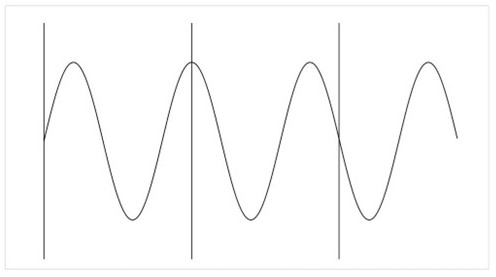
\includegraphics[width=.5\columnwidth]{img/12.jpg}
      \label{sub8}
    }~
    \subfigure[表示波形]{
    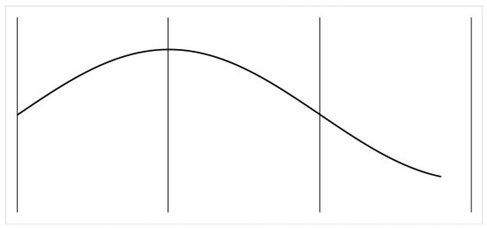
\includegraphics[width=.5\columnwidth]{img/13.jpg}
      \label{sub9}
    }
   \caption{フーリエ級数による近似}
   \label{im8}
   \end{center}
\end{figure}

追加検討1について、実験結果 (1)、実験結果 (2)、実験結果 (3) の実験において、
トリガレベルを正と負のピーク値の間とその間の外に設定した場合の、
ディジタルオシロスコープとアナログオシロスコープについて、
トリガ点は画面左端のままで行っていた。しかし、ディジタルオシロスコープについて、
トリガ点の位置を表示画面の左端以外にも設定できる。そこで、実験1において、
トリガ点を変更させたときの動作の推測とその理由について述べたいと思う。
実験結果 (1) ~ (3) において、トリガレベルを波形のピーク値の間、
トリガ点を横軸方向に移動させたとき、移動させた点から波形が表示される。
また、トリガ点以前の波形を表示させることができると推測できる。
その理由として、ディジタルオシロスコープは原理で述べたように、
ディジタル信号のデータをメモリに保存したのちに、波形を表示するため、
原理図\ref{im1}の演算部において保存されたトリガ点以前のデータを読み込むことによって、
画面にその部分の波形を表示させることができるからである。
一方アナログオシロスコープにおいて、トリガ点を変更することはできない。
なぜなら、ディジタルオシロスコープと違い、波形を保存することができないため、
現時点での波形しか表示できないので、トリガ点以前の現在よりも前の時間の波形を表示させることが
できないからである。従って、アナログオシロスコープにおいて、
トリガレベルを自由に設定できるがトリガポジションを自由に設定できない。
\par
追加検討2について、ディジタルオシロスコープの波形取り込みモードについて、
本実験においてはサンプルモードとアベレージモードにおいての表示波形の変化を観測したが、
アベレージモードは単発信号の波形取り込みができない。
なぜなら、連続波形の取り込みを複数回にわたって行い、波形を平均化して表示波形とするため、
単発信号では波形の表示を1度しかできないため波形の取り込みを1回しかできないからである。
また、アベレージモードの欠点を補うためのモードとして、ハイレゾモードが存在する。
ハイレゾモードとはサンプルモードであるときサンプリング間隔において、
一つのサンプリング間隔にさらに複数のサンプリングをしてそれらのサンプリングを平均し、
波形を表示するといったものになる。

\mysubsection{実験2}
実験結果 (2) において、表\ref{tb2}、 \ref{tb3} より、フーリエ係数$a_n$において、$n$ の値が大きくなるほど、
係数の値が小さくなっていることから、振幅の小さい正弦波の項が足されることによって、
元の波形の垂直成分を再現していることが推測される。
\par
$b_n$ において、$n$ の値が大きくなるほど係数の値が正と負を繰り返すことから、
正と負の振幅を足すことによって波形の垂直成分を定数に近づけて水平成分を平坦にし、
元の波形の水平成分を再現していることが推測される。
\par
実験結果 (3) において
表\ref{tb2}、\ref{tb3}と表\ref{tb4}、\ref{tb5}を比較して、
フーリエ級数 $b_3$, $b_6$, $a_3$, $a_6$ に大きな誤差も見られたが近似波形
図\ref{im8} と図 \ref{im8} は一致している。その理由として、式\eqref{eq5} において、
観測波形の振幅よりも小さい部分とそれよりも大きいとしている部分が相殺し、
近似波形が観測波形に近づいたと推測されるが、数値積分で計算した値の誤差を少なくするために、
標本化の時間間隔をより狭くするようなオシロスコープの設定をするとよい。
\par
フーリエ係数$b_0$について、
式\ref{eq2}を見ると、$b_0$ は観測波形のDC成分を表す。
参考として、フーリエ級数 (数値積分による計算) から$b_0$を引いた値を実験1
実験結果 (6)の時間間隔に対応させて波形を作ると、
入力結合を AC モードとしたときの波形であると推測できる。
(図\ref{im5}) その理由として、 AC モードは波形の正の値を表す面積と負の値を表す面積を等しくし、
観測波形のDC成分を0にするモードであるため、
フーリエ級数におけるDC成分の項$b_0$を0にすることによって、
DC モードの波形を AC モードの波形として描きかえることができるからである。

\newpage
\pagestyle{plain}
\bibliographystyle{jplain}
\addcontentsline{toc}{section}{参考文献}
\begin{thebibliography}{3}
\setlength{\parskip}{0cm} %enumerateのマージン
\setlength{\itemsep}{0cm}

\bibitem{repo}
東洋大学ホームページ 機械工学実験II補助資料実験レポートの書き方\\
URL: \verb|www2.toyo.ac.jp/~fujimatsu/kikai2/EXP_report.pdf|\\
参照年月日 平成30年4月22日

\bibitem{iwa}
岩崎 俊, 電子情報レクチャーシリーズB-13電磁気計測, コロナ社, 2002年8月30日発行

\bibitem{note}
電気電子計測講義ノート

\bibitem{slide}
電気情報工学実験II配布スライド
\bibitem{hyrezo}
オシロの「ハイレゾ」とは何か 日経xTECH (クロステック)\\
URL: \verb|http://nikkeibp.co.jp/dm/atcl/feature/15/032700084/032800015/| \\
参照年月日 平成30年5月19日


\end{thebibliography}

\end{document}